%%%%%%%%%%%%%%%%%%%%%%%%%%%%%%%%%%%%%%%%%
%
%%%%%%%%%%%%%%%%%%%%%%%%%%%%%%%%%%%%%%%%%


% REFERENCIAR IMAGENES: \autoref

\RequirePackage{silence}
\WarningFilter{soulutf8}{This package is obsolete}
\WarningFilter{scrreprt}{Usage of package `titlesec' together}
\WarningFilter{titlesec}{Non standard sectioning command}
\WarningFilter{scrreprt}{Usage of package `tocloft' together}

%----------------------------------------------------------------------------------------
%	PACKAGES AND OTHER DOCUMENT CONFIGURATIONS
%---------------------------------------------------------------------------------------- 
\documentclass[twoside, 
DIV = 10,
openright,titlepage,numbers=noenddot,headinclude,
headlines,footinclude=true,cleardoublepage=empty,paper=a4,fontsize=12pt, % Binding correction, paper type and font 
spanish, % Languages
]{scrreprt} 

% Includes the file which contains all the document configurations and packages - make sure to edit this file
% ============================================================
%   classicthesis-config.tex
%   Configuración del paquete classicthesis
% ============================================================

\PassOptionsToPackage{eulerchapternumbers,listings,pdfspacing,subfig,beramono,eulermath,dottedtoc}{classicthesis}

% ------------------------------------------------------------
%   INFORMACIÓN DEL DOCUMENTO
% ------------------------------------------------------------

\newcommand{\myTitle}{VICON: Sistema de Visión configurable\xspace}
\newcommand{\mySubtitle}{\xspace}
\newcommand{\myName}{Carlos Manuel Gómez Jiménez\xspace}
\newcommand{\mySupervisor}{Martín González García\xspace}
\newcommand{\myDepartment}{Departamento de Ingeniería Informática y de Sistemas\xspace}
\newcommand{\myUni}{Universidad de Málaga\xspace}
\newcommand{\myLocation}{Málaga\xspace}
\newcommand{\myTime}{Septiembre 2026\xspace}
\newcommand{\myVersion}{version 1.0\xspace}

% ------------------------------------------------------------
%   COMANDOS ÚTILES
% ------------------------------------------------------------

\newcommand{\ie}{i.\,e.}
\newcommand{\Ie}{I.\,e.}
\newcommand{\eg}{e.\,g.}
\newcommand{\Eg}{E.\,g.}

\newcounter{dummy} % Necesario para hipervínculos correctos (índice, bibliografía, etc.)

% ------------------------------------------------------------
%   PAQUETES BÁSICOS
% ------------------------------------------------------------

\usepackage[utf8]{inputenc}
\usepackage[T1]{fontenc}
\usepackage{xspace}

\PassOptionsToPackage{spanish,es-lcroman,es-tabla}{babel}
\usepackage{babel}

\PassOptionsToPackage{square,numbers}{natbib}
\usepackage{natbib}

\PassOptionsToPackage{fleqn}{amsmath}
\usepackage{amsmath}

\PassOptionsToPackage{pdftex}{graphicx}
\usepackage{graphicx}

% Comando para limpiar hasta página izquierda
\newcommand*\cleartoleftpage{%
  \clearpage
  \ifodd\value{page}\hbox{}\newpage\fi
}

% ------------------------------------------------------------
%   TABLAS, FIGURAS Y CAPTIONS
% ------------------------------------------------------------

\usepackage{tabularx}
\setlength{\extrarowheight}{3pt}
\newcommand{\tableheadline}[1]{\multicolumn{1}{c}{\spacedlowsmallcaps{#1}}}
\newcommand{\myfloatalign}{\centering}
\usepackage{caption}
\captionsetup{format=hang,font=small}
\usepackage{subfig}
\usepackage{floatrow}
\floatsetup[table]{capposition=top}

% ------------------------------------------------------------
%   LISTINGS (CÓDIGO FUENTE)
% ------------------------------------------------------------

\usepackage{listings}
\lstset{
  language=[LaTeX]Tex,
  keywordstyle=\color{RoyalBlue},
  basicstyle=\small\ttfamily,
  commentstyle=\color{Green}\ttfamily,
  stringstyle=\rmfamily,
  numbers=left,
  numberstyle=\scriptsize,
  stepnumber=5,
  numbersep=8pt,
  showstringspaces=false,
  breaklines=true,
  frame=single,
  belowcaptionskip=.75\baselineskip
}

% ------------------------------------------------------------
%   HIPERVÍNCULOS
% ------------------------------------------------------------

\PassOptionsToPackage{pdftex,hyperfootnotes=false,pdfpagelabels,colorlinks=true,allcolors=black}{hyperref}
\usepackage{hyperref}



\pdfcompresslevel=9
\pdfadjustspacing=1

\hypersetup{
  colorlinks=true,
  pdfstartpage=1,
  pdfstartview=FitV,
  breaklinks=true,
  pdfpagemode=UseOutlines,
  pageanchor=true,
  plainpages=false,
  bookmarksnumbered,
  bookmarksopen=true,
  bookmarksopenlevel=1,
  hypertexnames=true,
  pdfhighlight=/O,
  urlcolor=webbrown,
  linkcolor=blue,
  citecolor=black,
  linktoc=all,
  % Metadatos PDF
  pdftitle={\myTitle},
  pdfauthor={\textcopyright\ \myName, \myUni},
  pdfcreator={pdfLaTeX},
  pdfproducer={LaTeX with hyperref and classicthesis}
}


\PassOptionsToPackage{smaller}{acronym}
\usepackage{acronym}
\providecommand{\bflabel}{}
\renewcommand{\bflabel}[1]{{#1}\hfill}


% ------------------------------------------------------------
%   AUTORREFERENCIAS (español)
% ------------------------------------------------------------

\makeatletter
\@ifpackageloaded{babel}{
  \addto\extrasspanish{
    \renewcommand*{\figureautorefname}{Figura}
    \renewcommand*{\tableautorefname}{Tabla}
    \renewcommand*{\partautorefname}{Parte}
    \renewcommand*{\chapterautorefname}{Capítulo}
    \renewcommand*{\sectionautorefname}{Sección}
    \renewcommand*{\subsectionautorefname}{Sección}
    \renewcommand*{\subsubsectionautorefname}{Sección}
  }
  \providecommand{\subfigureautorefname}{\figureautorefname}
}{\relax}
\makeatother

% ------------------------------------------------------------
%   CLASSICTHESIS Y PAQUETES ADICIONALES
% ------------------------------------------------------------

\usepackage{classicthesis}
\usepackage[textwidth=25mm]{todonotes}
%\usepackage[textwidth=25mm,disable]{todonotes}
\usepackage{subfiles}
\usepackage{soulutf8}

\newcommand{\todosolve}[2][]{\todo[color=green!50,size=\tiny,#1]{#2}}
\newcommand{\todohint}[2][]{\todo[color=yellow!50,size=\tiny,#1]{#2}}

\makeatletter
\if@todonotes@disabled
  \newcommand{\hlfix}[2]{#1}
\else
  \newcommand{\hlfix}[2]{\texthl{#1}\todo{#2}}
\fi
\makeatother

\usepackage{pdfpages}
\usepackage{lscape}
\usepackage{multirow}
\usepackage{siunitx}
\usepackage{booktabs}
\usepackage{hyphenat}
\usepackage{placeins}
\usepackage[numbered,framed]{matlab-prettifier}
\usepackage{colortbl}
\definecolor{LightCyan}{rgb}{0,0.5,1}
\usepackage[official]{eurosym}
\usepackage{bigstrut}
\usepackage{adjustbox}
\usepackage{gensymb}
\usepackage[margin=2.5cm,top=2.5cm,bottom=2.5cm]{geometry}
\usepackage{makecell}

\usepackage[most]{tcolorbox}

\tcbuselibrary{skins, breakable}
 
\definecolor{reqblue}{HTML}{156082}
 
\newtcolorbox{requisito}[2]{
    enhanced,
    breakable,
    colback       = white,
    colframe      = reqblue,
    colbacktitle  = reqblue,
    coltitle      = white,
    fonttitle     = \bfseries\small,
    title         = {#1 \hfill #2},
    left          = 4pt,
    right         = 4pt,
    top           = 2pt,
    bottom        = 2pt,
    boxrule       = 0.8pt,
    arc           = 2pt,
} 

\usepackage{longtable}
\usepackage{svg}
\usepackage{placeins}

\titleformat{\chapter}[display]
  {\normalfont\large\scshape}
  {\raggedleft\color{halfgray}\fontsize{60}{60}\selectfont\thechapter} % Número/Letra alineado dentro del margen
  {-10pt} % Espacio entre la 'A' y el título
  {\raggedright\spacedallcaps}[\vspace*{0.8ex}\titlerule] % Título en versalitas y la línea debajo (\titlerule)

% Ajusta el espacio en blanco de arriba y abajo
% \titlespacing*{<comando>}{<izquierda>}{<arriba>}{<abajo>}
\titlespacing*{\chapter}{0pt}{5pt}{30pt}
\begin{document}

	\frenchspacing % Reduces space after periods to make text more compact
	\raggedbottom % Makes all pages the height of the text on that page
	\selectlanguage{spanish} % Select your default language - e.g. american or ngerman
	
	%\renewcommand*{\bibname}{new name} % Uncomment to change the name of the bibliography
	%\setbibpreamble{} % Uncomment to include a preamble to the bibliography - some text before the reference list starts
	
	\pagenumbering{roman} % Roman page numbering prior to the start of the thesis content (i, ii, iii, etc)
	\pagestyle{plain} % Suppress headers for the pre-content pages
	\cleardoublepage% !TEX encoding = latin9
\begin{titlepage}
    \begin{center}
        \large
        \hfill
        \vfill
        
        {\huge\scshape Universidad de Málaga \par}
        \vspace{0.4cm}
        {\Large\scshape Escuela Técnica Superior de Ingeniería de Telecomunicación \par}        
        \vspace{1.5cm}
        
        % Logo de la Universidad
		\vspace{0.8cm} % Reducido para que quepa todo
        
        % Contenedor de logos alineados
        \noindent
        \begin{minipage}[c]{0.45\textwidth}
            \centering
            
\includegraphics[height=2.2cm]{gfx/logo_uma_1} 
        \end{minipage}
        \hfill
        \begin{minipage}[c]{0.45\textwidth}
            \centering
            
\includegraphics[height=2.2cm]{gfx/logo_uma_2} 
        \end{minipage}
        
        \vspace{0.8cm}
        
        {\Large\bfseries TRABAJO FIN DE MÁSTER \par}
        
        \vspace{1cm}
        
        % Titulo del proyecto
        {\huge\bfseries \myTitle \par}
        
        \vspace{1cm}
        
        % Nombre del Master
        {\Large Máster en Sistemas Electrónicos \\ para Entornos Inteligentes \par}        
        \vspace{2cm}
        
        {\Large MÁLAGA, 2026 \par} 
        
        \vspace{1.5cm}
        
        {\Large \myName \par}
        
        \vfill
    \end{center}
\end{titlepage}

\cleardoublepage

\begin{titlepage}
    \begin{center}
        {\large\scshape Universidad de Málaga \par}
        \vspace{0.2cm}
        {\normalsize\scshape Escuela Técnica Superior de Ingeniería de Telecomunicación \par}        
        \vspace{1.5cm}
        
        {\Large\bfseries \myTitle \par}
        
        \vspace{1.5cm}
    \end{center}
    
    \noindent\textbf{REALIZADO POR:}\\
    \myName
    
    \vspace{0.8cm}
    
    \noindent\textbf{DIRIGIDO POR:}\\
    \mySupervisor
    
    \vspace{0.8cm}
    
    \noindent\textbf{DEPARTAMENTO:}\\
    Departamento de Tecnolog{\'i}a Electr{\'o}nica
    
    \vspace{0.8cm}
    
    \noindent\textbf{TITULACI{\'O}N:}\\
    M{\'a}ster en Sistemas Electr{\'o}nicos para Entornos Inteligentes
    
    \vspace{0.8cm}
    
    \noindent\textbf{PALABRAS CLAVE:}\\
    FPGA, VHDL, RTL, Síntesis Lógica, sensor CMOS, visión artificial, OpenCV.
    
    \vspace{0.8cm}
    
    %\noindent\textbf{RESUMEN:}\\
    %Este proyecto consiste en el estudio del funcionamiento del m{\'o}dulo sensor...
    
    \vfill
    
    \begin{flushright}
        M{\'a}laga, \today
    \end{flushright}
\end{titlepage} % Main title page
	%
\includepdf[pages=-]{gfx/thesis-front-cover.pdf}
	\cleardoublepage\include{FrontBackMatter/Titleback} % Back of the title page
	%1\cleardoublepage\include{FrontBackMatter/Dedication} % Dedication page
	%1\cleardoublepage\include{FrontBackMatter/Foreword} % Uncomment and create a Foreword.tex to include a foreword
	\cleardoublepage% Abstract

\pdfbookmark[1]{Resumen}{Resumen} % Bookmark name visible in a PDF viewer

% \begingroup
% \let\clearpage\relax
% \let\cleardoublepage\relax
% \let\cleardoublepage\relax




\chapter*{Resumen} % Abstract name

Este trabajo presenta el diseño, implementación y verificación de VICON, un sistema de adquisición y transmisión de imagen en tiempo 
real basado en FPGA. El sistema integra el sensor de imagen CMOS MT9V111 con la plataforma Basys~3 (Xilinx Artix-7) y transmite el flujo de vídeo hacia un PC mediante 
el chip FT232H de FTDI operando en modo \textit{Synchronous FIFO} sobre un enlace de 60~MHz.
El diseño hardware, desarrollado íntegramente en VHDL, comprende un controlador I2C para la configuración del sensor, un módulo de captura de trama con gestión 
de marcadores de protocolo, un controlador de alta velocidad para el FT232H con arquitectura de doble proceso para TX y RX, y un procesador de comandos con 
sincronización entre dominios de reloj (CDC). La verificación se realiza mediante simulación y con pruebas en Hardware, 
en la primera empleando agentes para el sensor I2C y para el chip FT232H. El software de visualización, desarrollado en C++ con Qt y OpenCV, recibe el flujo de imagen y permite enviar comandos de control a la FPGA.
El sistema completo ha sido validado sobre hardware real, demostrando la transmisión de imagen en escala de grises a resolución VGA (640$\times$480) y la correcta ejecución de todos los comandos de control.

% \par\vfill\pagebreak


\pdfbookmark[1]{Abstract}{Abstract} % Bookmark name visible in a PDF viewer

\chapter*{Abstract} % Abstract name

This work presents the design, implementation and verification of VICON, a real-time image acquisition and transmission system based on FPGA. The system integrates the CMOS image sensor MT9V111 with the Basys~3 platform (Xilinx Artix-7) and transmits the video stream to a PC through the FTDI FT232H chip, operating in \textit{Synchronous FIFO} mode over a 60~MHz link. The hardware design, developed entirely in VHDL, comprises an I2C controller for sensor configuration, a frame capture module with protocol marker handling, a high-speed controller for the FT232H featuring a dual-process architecture for TX and RX, and a command processor with clock domain crossing (CDC) synchronisation. Verification is carried out through simulation and hardware testing; the former employs UVVM-based agents for both the I2C sensor and the FT232H chip. The visualisation software, developed in C++ with Qt and OpenCV, receives the image stream and allows control commands to be sent to the FPGA. The complete system has been validated on real hardware, demonstrating the transmission of grayscale images at VGA resolution (640$\times$480) and the correct execution of all control commands.


% \endgroup
\providecommand{\keywords}[1]
{
	\small	
	\textbf{\textit{Keywords---}} #1

}			

\vfill % Abstract page
	%1\cleardoublepage\include{FrontBackMatter/Publication} % Publications from the thesis page
	\cleardoublepage% Acknowledgements

\pdfbookmark[1]{Agradecimientos}{Agradecimientos} % Bookmark name visible in a PDF viewer


\bigskip

%----------------------------------------------------------------------------------------

\begingroup

\let\clearpage\relax
\let\cleardoublepage\relax
\let\cleardoublepage\relax

\chapter*{Agradecimientos} % Acknowledgements section text

Quiero agradecer en primer lugar a mi tutor, por su disponibilidad, sus comentarios y la orientación prestada durante el desarrollo de este trabajo.

A mi familia y a Desi, por su apoyo y paciencia a lo largo de todos los altibajos de este proceso.

\endgroup % Acknowledgements page
	\pagestyle{scrheadings} % Show chapter titles as headings
	\cleardoublepage% Table of Contents - List of Tables/Figures/Listings and Acronyms 

\refstepcounter{dummy}

\pdfbookmark[1]{\contentsname}{tableofcontents} % Bookmark name visible in a PDF viewer

\setcounter{tocdepth}{2} % Depth of sections to include in the table of contents - currently up to sections

\setcounter{secnumdepth}{3} % Depth of sections to number in the text itself - currently up to subsubsections

\manualmark
\markboth{\spacedlowsmallcaps{\contentsname}}{\spacedlowsmallcaps{\contentsname}}
\tableofcontents 
\automark[section]{chapter}
\renewcommand{\chaptermark}[1]{\markboth{\spacedlowsmallcaps{#1}}{\spacedlowsmallcaps{#1}}}
\renewcommand{\sectionmark}[1]{\markright{\thesection\enspace\spacedlowsmallcaps{#1}}}

\clearpage

\begingroup 
\let\clearpage\relax
\let\cleardoublepage\relax
\let\cleardoublepage\relax

%----------------------------------------------------------------------------------------
%	List of Figures
%----------------------------------------------------------------------------------------

%\refstepcounter{dummy}
%\addcontentsline{toc}{chapter}{\listfigurename} % Uncomment if you would like the list of figures to appear in the table of contents
%\pdfbookmark[1]{\listfigurename}{lof} % Bookmark name visible in a PDF viewer

%\listoffigures

%\vspace*{8ex}
%\newpage

%----------------------------------------------------------------------------------------
%	List of Tables
%----------------------------------------------------------------------------------------

%\refstepcounter{dummy}
%\addcontentsline{toc}{chapter}{\listtablename} % Uncomment if you would like the list of tables to appear in the table of contents
%\pdfbookmark[1]{\listtablename}{lot} % Bookmark name visible in a PDF viewer

%\listoftables
        
        %\vspace*{8ex}
        %\newpage
            
            %----------------------------------------------------------------------------------------
            %	List of Listings
            %---------------------------------------------------------------------------------------- 

            %\refstepcounter{dummy}
            %\addcontentsline{toc}{chapter}{\lstlistlistingname} % Uncomment if you would like the list of listings to appear in the table of contents
            %\pdfbookmark[1]{\lstlistlistingname}{lol} % Bookmark name visible in a PDF viewer

            %\lstlistoflistings 
            %\todo{Quitar esto no?}
            %\vspace*{8ex}
            %\newpage
             
            % \pdfbookmark[1]{Lista de TODOS}{todolist}
	        % \listoftodos  
            % \newpage

            \newpage
            \thispagestyle{empty}
            \mbox{}
            \newpage

            \pdfbookmark[1]{Lista de Figuras}{figurelist}
	        \listoffigures 
            \newpage

            \newpage
            \thispagestyle{empty}
            \mbox{}
            \newpage

            \pdfbookmark[1]{Lista de Tablas}{tablelist}
	        \listoftables 
            \newpage
             %----------------------------------------------------------------------------------------
             %	Acronyms
             %----------------------------------------------------------------------------------------
             
            \newpage
            \thispagestyle{empty}
            \mbox{}
            \newpage

             \refstepcounter{dummy}
             %\addcontentsline{toc}{chapter}{Acronyms} % Uncomment if you would like the acronyms to appear in the table of contents
             \pdfbookmark[1]{Acrónimos}{Acrónimos} % Bookmark name visible in a PDF viewer

             \markboth{\spacedlowsmallcaps{Acronyms}}{\spacedlowsmallcaps{Acronyms}}
             \chapter*{Acronimos}

             \begin{acronym}[UML]
             \acro{PCB}{Printed Circuit Board}
             \acro{VGA}{Video Graphics Array}
             \acro{FPGA}{Field-Programmable Gate Array}
             \acro{VHDL}{VHSIC Hardware Description Language}
             \acro{CDC}{Clock Domain Crossing}
             \acro{UVVM}{Universal VHDL Verification Methodology}
             \acro{TFM}{Trabajo Fin de Máster}
             \acro{VICON}{Sistema de Visión Configurable}
             \acro{RTL}{Register Transfer Level}
             \acro{FIFO}{First In - First Out}
             \acro{SW}{Software}
             \acro{HW}{Hardware}
             \acro{TB}{TestBench}
             \acro{VVC}{VHDL Verification Component}
             \acro{UVM}{Universal Verification Methodology}
             \acro{OSVVM}{Open Source VHDL Verification Methodology}
             \acro{ILA}{Integrated Logic Analyzer}
             \acro{IP}{Intellectual Property}
             \acro{IDE}{Entorno de Desarrollo Integrado}
             \acro{IFP}{Image Flow Processor}
             \acro{FPS}{Frames por segundo}
             \acro{SCL}{Serial Clock}
             \acro{SDA}{Serial Data}
             \acro{FSM}{Finite State Machine}
             \acro{MMCM}{Mixed-Mode Clock Manager}
             \acro{GUI}{Graphical User Interface}
             \acro{FWFT}{First Word Fall Through}
             \acro{I2C}{Inter-Integrated Circuit}
             \acro{DUT}{Device Under Test}
             \acro{CCIO}{Clock Capable Input/Output}
             \acro{LUT}{Look Up Table}
             \acro{IOB}{Input/Output Block}
             \acro{PS}{Processing System}
             \acro{ACK}{Acknowledge}
             \acro{EEPROM}{Electrically Erasable Programmable Read-Only Memory}
             \acro{SBC}{Single Board Computer}
             \acro{PLL}{Phase-locked loop}
             \end{acronym}  
\endgroup    % Contents, list of figures/tables/listings and acronyms
	\cleardoublepage 
	\pagenumbering{arabic} % Arabic page numbering for thesis content (1, 2, 3, etc)
	%\setcounter{page}{90} % Uncomment to manually start the page counter at an arbitrary value (for example if you wish to count the pre-content pages in the page count)

	\cleardoublepage % Avoids problems with pdfbookmark
	
	%----------------------------------------------------------------------------------------
	%	THESIS CONTENT - CHAPTERS
	%----------------------------------------------------------------------------------------
	
	%1\ctparttext{You can put some informational part preamble text here. Illo principalmente su nos. Non message \emph{occidental} angloromanic da. Debitas effortio simplificate sia se, auxiliar summarios da que, se avantiate publicationes via. Pan in terra summarios, capital interlingua se que. Al via multo esser specimen, campo responder que da. Le usate medical addresses pro, europa origine sanctificate nos se.} % Text on the Part 1 page describing  the content in Part 1
	
	%1\part{Some Kind of Manual} % First part of the thesis


	\subfile{Chapters/cap_introduccion.tex}

	\subfile{Chapters/cap_estado_arte.tex}

	\subfile{Chapters/cap_herramientas.tex}

	\subfile{Chapters/cap_requisitos.tex}

	\subfile{Chapters/cap_descripcion_sistema.tex}

	\subfile{Chapters/cap_desarrollo.tex}

	\subfile{Chapters/cap_software.tex}

	\subfile{Chapters/cap_implementacion.tex}

	\subfile{Chapters/cap_resultados.tex}

	\subfile{Chapters/cap_conclusiones.tex}

	
	
	%----------------------------------------------------------------------------------------
	%	THESIS CONTENT - APPENDICES
	%----------------------------------------------------------------------------------------
	\cleardoublepage
    \include{FrontBackMatter/Bibliography} % Bibliography
	%\appendix
	%\pagenumbering{gobble}
	%1\part{Appendix} % New part of the thesis for the appendix
    %\chapter{Manual de Usuario}
\label{ch:manual_usuario}

En este apéndice se detalla el manual de usuario correspondiente al sistema desarrollado, guiando paso a paso en el proceso de uso de la plataforma. Se asume que la \ac{FPGA} ya tiene el diseño programado en su memoria de configuración; este manual cubre por tanto la puesta en marcha del hardware y el uso del software de PC.

% -----------------------------------------------------------------
\section{Requisitos del sistema}
\label{sec:requisitos}

Antes de iniciar la instalación, hay que cumplir con los siguientes requisitos previos en su equipo:

\begin{itemize}
    \item \textbf{Sistema operativo:} Windows~11, con un mínimo de 8~GB de RAM.
    \item \textbf{Basys~3:} Basys~3 con el \textit{bitstream} de VICON ya programado en su memoria de configuración, conectada al sensor MT9V111 y al chip FT232H (módulo UM232H-B) utilizando los conectores \textit{Pmod} indicados en la Figura~\ref{fig:arq_fisica}.
    \item \textbf{Driver D2XX:} controlador D2XX de FTDI instalado en el PC (disponible en \url{https://ftdichip.com/drivers/d2xx-drivers/}), necesario para que la aplicación de PC acceda al FT232H.
    \item \textbf{Cable USB:} un cable USB~2.0 que conecte el módulo UM232H-B directamente a un puerto del PC. Se recomienda evitar conectarlo a través de un \textit{hub} USB, ya que puede introducir latencias adicionales en la recepción del vídeo.
\end{itemize}

\textit{Antes de encender o alimentar la placa}, comprobar la posición del \textit{jumper} de modo de arranque (\texttt{JP1}). Para que la Basys~3 cargue el diseño desde su memoria de configuración no volátil, dicho \textit{jumper} debe situarse en la posición \texttt{QSPI}; en la posición \texttt{USB} la placa esperaría en su lugar una programación por JTAG desde Vivado.

% -----------------------------------------------------------------
\section{Instalación y configuración}
\label{sec:instalacion}

Se deben seguir los pasos descritos a continuación para preparar el software de visualización:

\subsection{Descarga del código fuente}
Clonar el repositorio oficial del proyecto desde \url{https://github.com/carlosmgj/VICON}

\subsection{Configuración del módulo FT232H}
El módulo UM232H-B debe tener su \ac{EEPROM} configurada en modo \textbf{FT245 FIFO} para poder operar en modo \textit{Synchronous FIFO}. Esta configuración solo es necesaria una vez por dispositivo:

\begin{enumerate}
    \item Instalar la utilidad \textbf{FT\_Prog} de FTDI (requiere el driver D2XX ya instalado).
    \item Conectar el UM232H-B al PC y, en FT\_Prog, pulsar \textit{Scan and Parse} para detectar el dispositivo.
    \item Navegar hasta \texttt{FT EEPROM~$\rightarrow$~Hardware Specific~$\rightarrow$~Port~A~$\rightarrow$~Hardware} y cambiar el modo de \texttt{UART} a \texttt{245~FIFO}.
    \item Programar la \ac{EEPROM} (icono del rayo) y, al finalizar, desconectar y vuelva a conectar el módulo para que el sistema operativo lo reconozca con la nueva configuración.
\end{enumerate}

\subsection{Compilación de la aplicación de PC}
La aplicación \texttt{vicon\_view} se distribuye como un ejecutable y por tanto no hace falta tener las dependencias instaladas. Únicamente serían necesarias para la compilación de la aplicación.
La ruta del ejecutable es: \url{VICON/07-Versions/3.0/GUI/vicon_gui.exe}
% -----------------------------------------------------------------
\section{Guía de uso de la aplicación}
\label{sec:guia_uso}

\subsection{Inicio de la aplicación}
Con la Basys~3 encendida, el sensor conectado y el módulo FT232H enlazado al PC por USB, ejecutar \texttt{vicon\_view}. La aplicación abre el dispositivo FT232H a través del \textit{driver} D2XX y comienza a recibir el flujo de vídeo sintético de forma automática; no es necesario ningún paso adicional de emparejamiento o configuración del enlace.

\subsection{Descripción de la interfaz}
Una vez iniciada la interfaz de usuario, se presentan dos zonas principales:

\begin{enumerate}
    \item \textbf{Ventana de vídeo:} muestra en tiempo real el fotograma recibido desde la \ac{FPGA} en escala de grises, junto con la tasa de fotogramas por segundo (\ac{FPS}) actual.
    \item \textbf{Panel de control:} Se encuentran los controles para enviar comandos a la \ac{FPGA}, descritos en la Tabla~\ref{tab:comandos_gui}.
\end{enumerate}

Por defecto, la interfaz muestra el video sintético generado para validar la comunicación entre el sensor y el Host a través de la FPGA como se ve en la Figura~\ref{fig:GUI1}:

\begin{figure}[htbp]
    \centering
    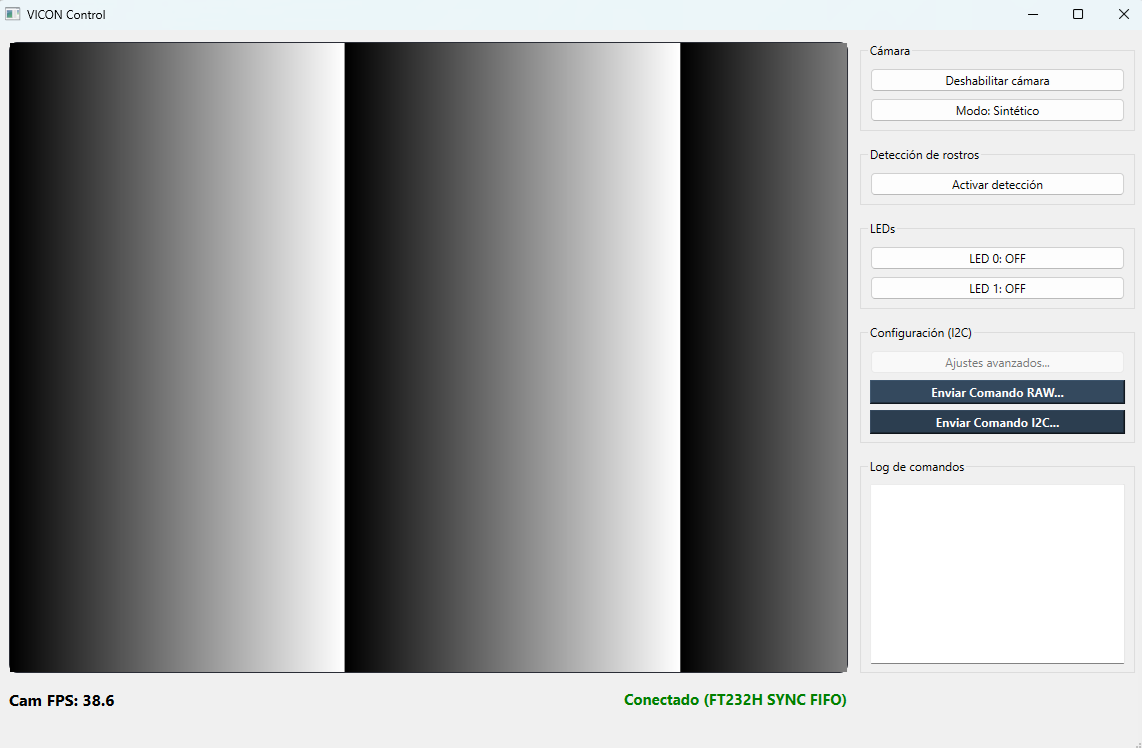
\includegraphics[width=\textwidth]{gfx/vicon_view_gui1.png}
    \caption{Estado Inicial de la Interfaz Gráfica de Usuario.}
    \label{fig:GUI1}
\end{figure}

Para configurar los FPS de la imágen a mínimo 30fps, se deberá configurar el registro I2C correspondiente mandando la trama 1 0x37 0x0080 (Ver Figura~\ref{fig:GUI2}). Este paso se puede realizar antes o después de cambiar el modo de la imágen. 

\begin{figure}[htbp]
    \centering
    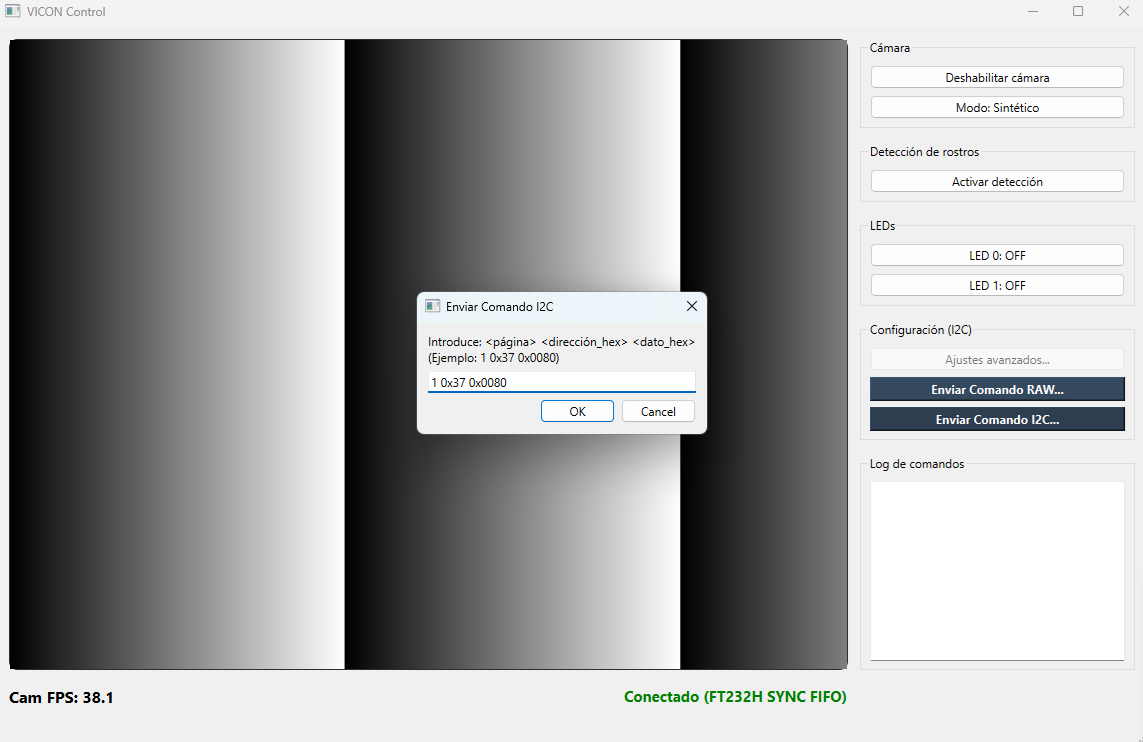
\includegraphics[width=\textwidth]{gfx/vicon_view_gui2.png}
    \caption{GUI: envío de comando I2C para configurar >30fps.}
    \label{fig:GUI2}
\end{figure}

Si a continuación habilitamos la imagen del sensor real y la detección de rostros, el software remarcara la/s cara/s que detecte en la imagen. En la Figura~\ref{fig:GUI3} se puede ver el resultado de presentar al sensor una foto en una tablet con múltiples caras. 

\begin{figure}[htbp]
    \centering
    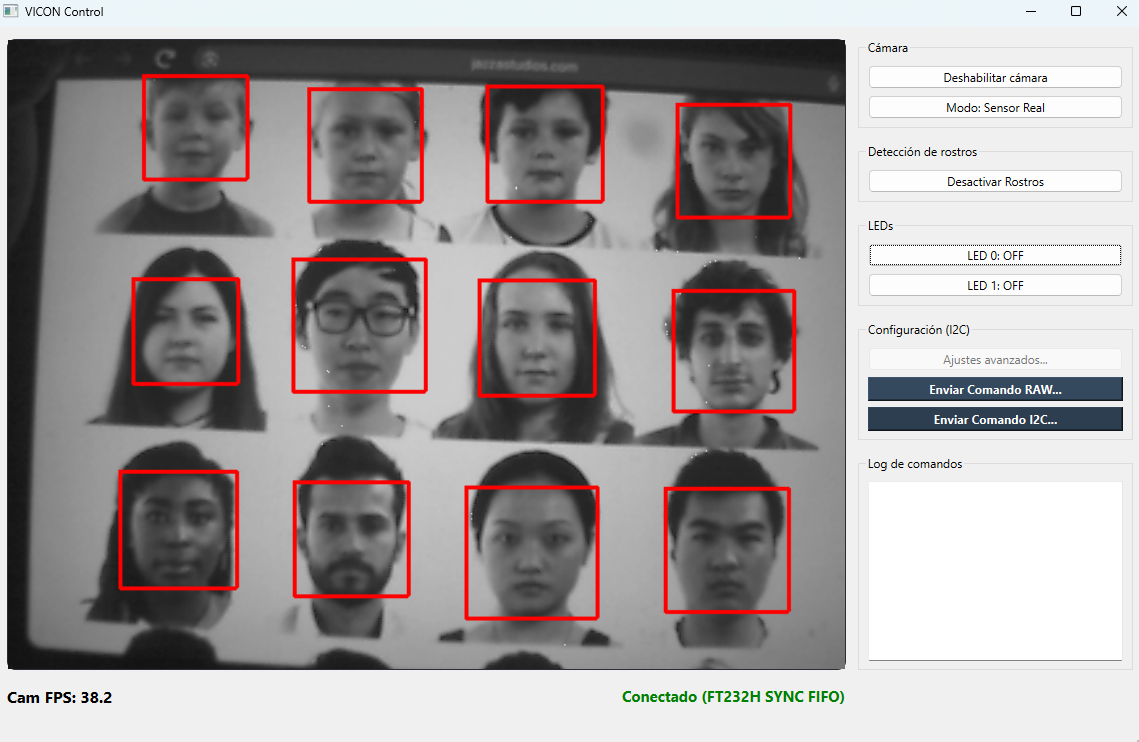
\includegraphics[width=\textwidth]{gfx/vicon_view_gui3.png}
    \caption{GUI: envío de comando I2C para configurar >30fps.}
    \label{fig:GUI3}
\end{figure}

\begin{table}[H]
\centering
\caption{Comandos disponibles desde la interfaz de \texttt{vicon\_view}.}
\label{tab:comandos_gui}
\begin{tabular}{>{\raggedright\arraybackslash}p{3cm}>{\raggedright\arraybackslash}p{9.5cm}}
\rowcolor[HTML]{156082}
{\color{white}\textbf{Comando}} & {\color{white}\textbf{Efecto}} \\
\rowcolor[HTML]{C0E6F5}
LED & Conmuta el estado de un LED de la Basys~3, útil como comprobación rápida de que el canal de comandos PC$\rightarrow$FPGA funciona. \\
Activar/desactivar captura & Detiene o reanuda la transmisión de vídeo desde la \ac{FPGA} sin necesidad de desconectar el enlace USB. \\
\rowcolor[HTML]{C0E6F5}
Imagen sintética & Conmuta entre el sensor MT9V111 y el generador interno de imagen sintética, útil para validar el resto de la cadena sin depender de la cámara física. \\
Escritura de registro I2C & Permite escribir un valor en un registro concreto del sensor (página, dirección y dato), para ajustar su configuración en caliente. \\
\end{tabular}
\end{table}

% -----------------------------------------------------------------
\section{Resolución de problemas (\textit{troubleshooting})}
\label{sec:problemas}

En la Tabla~\ref{tab:errores_frecuentes} se resumen los errores más habituales y las acciones recomendadas para su resolución.

\begin{table}[htbp]
\centering
\caption{Problemas frecuentes y soluciones.}
\label{tab:errores_frecuentes}
\begin{tabular}{|p{3.8cm}|p{4.6cm}|p{4.6cm}|}
\hline
\rowcolor[HTML]{156082}
{\color{white}\textbf{Error}} & {\color{white}\textbf{Causa probable}} & {\color{white}\textbf{Solución recomendada}} \\ \hline
No se ven los LEDs encendidos al arrancar la placa. & \textit{Jumper} de modo mal colocado. & Situar el \textit{jumper} \texttt{JP1} en modo \texttt{QSPI} antes de alimentar la placa. \\ \hline
La aplicación no detecta el FT232H. & Windows ha instalado automáticamente el \textit{driver} VCP (puerto serie virtual) en lugar del D2XX. & Reinstalar el \textit{driver} D2XX desde el Administrador de dispositivos, seleccionando manualmente la carpeta de instalación de FTDI. \\ \hline
FT\_Prog no reconoce el dispositivo al configurar la \ac{EEPROM}. & Conflicto entre el \textit{driver} D2XX y otro \textit{driver} (p.~ej. \texttt{libusb}) instalado previamente sobre el mismo dispositivo. & Reinstalar el \textit{driver} D2XX y volver a conectar el cable antes de reintentar con FT\_Prog. \\ \hline
El vídeo se congela o aparecen fotogramas corruptos de forma intermitente. & Sobreescritura de la \ac{FIFO} interna por una latencia de lectura excesiva en el PC (agravada si el FT232H está conectado a través de un \textit{hub} USB). & Conectar el módulo directamente a un puerto USB del equipo, sin \textit{hubs} intermedios. \\ \hline
\end{tabular}
\end{table} % Appendix A
	%\chapter{Diagramas de estados (FSM)}
\label{ch:anexo_fsm}

Este anexo recoge los diagramas de estados completos de las máquinas de estados finitas (\ac{FSM}) más voluminosas del diseño, referenciadas desde sus respectivos módulos en el Capítulo~\ref{chap:desarrollo}. Se han trasladado aquí, en lugar de incluirse en el cuerpo del documento, debido a su tamaño.

% -----------------------------------------------------------------
\section{FSM de configuración del TOP}
\label{sec:anexo_fsm_top}

Diagrama de estados de la FSM principal \texttt{p\_fsm} (\texttt{TOP.vhd}), descrita textualmente en la Sección~\ref{sec:top}.

\begin{figure}[htbp]
    \centering
    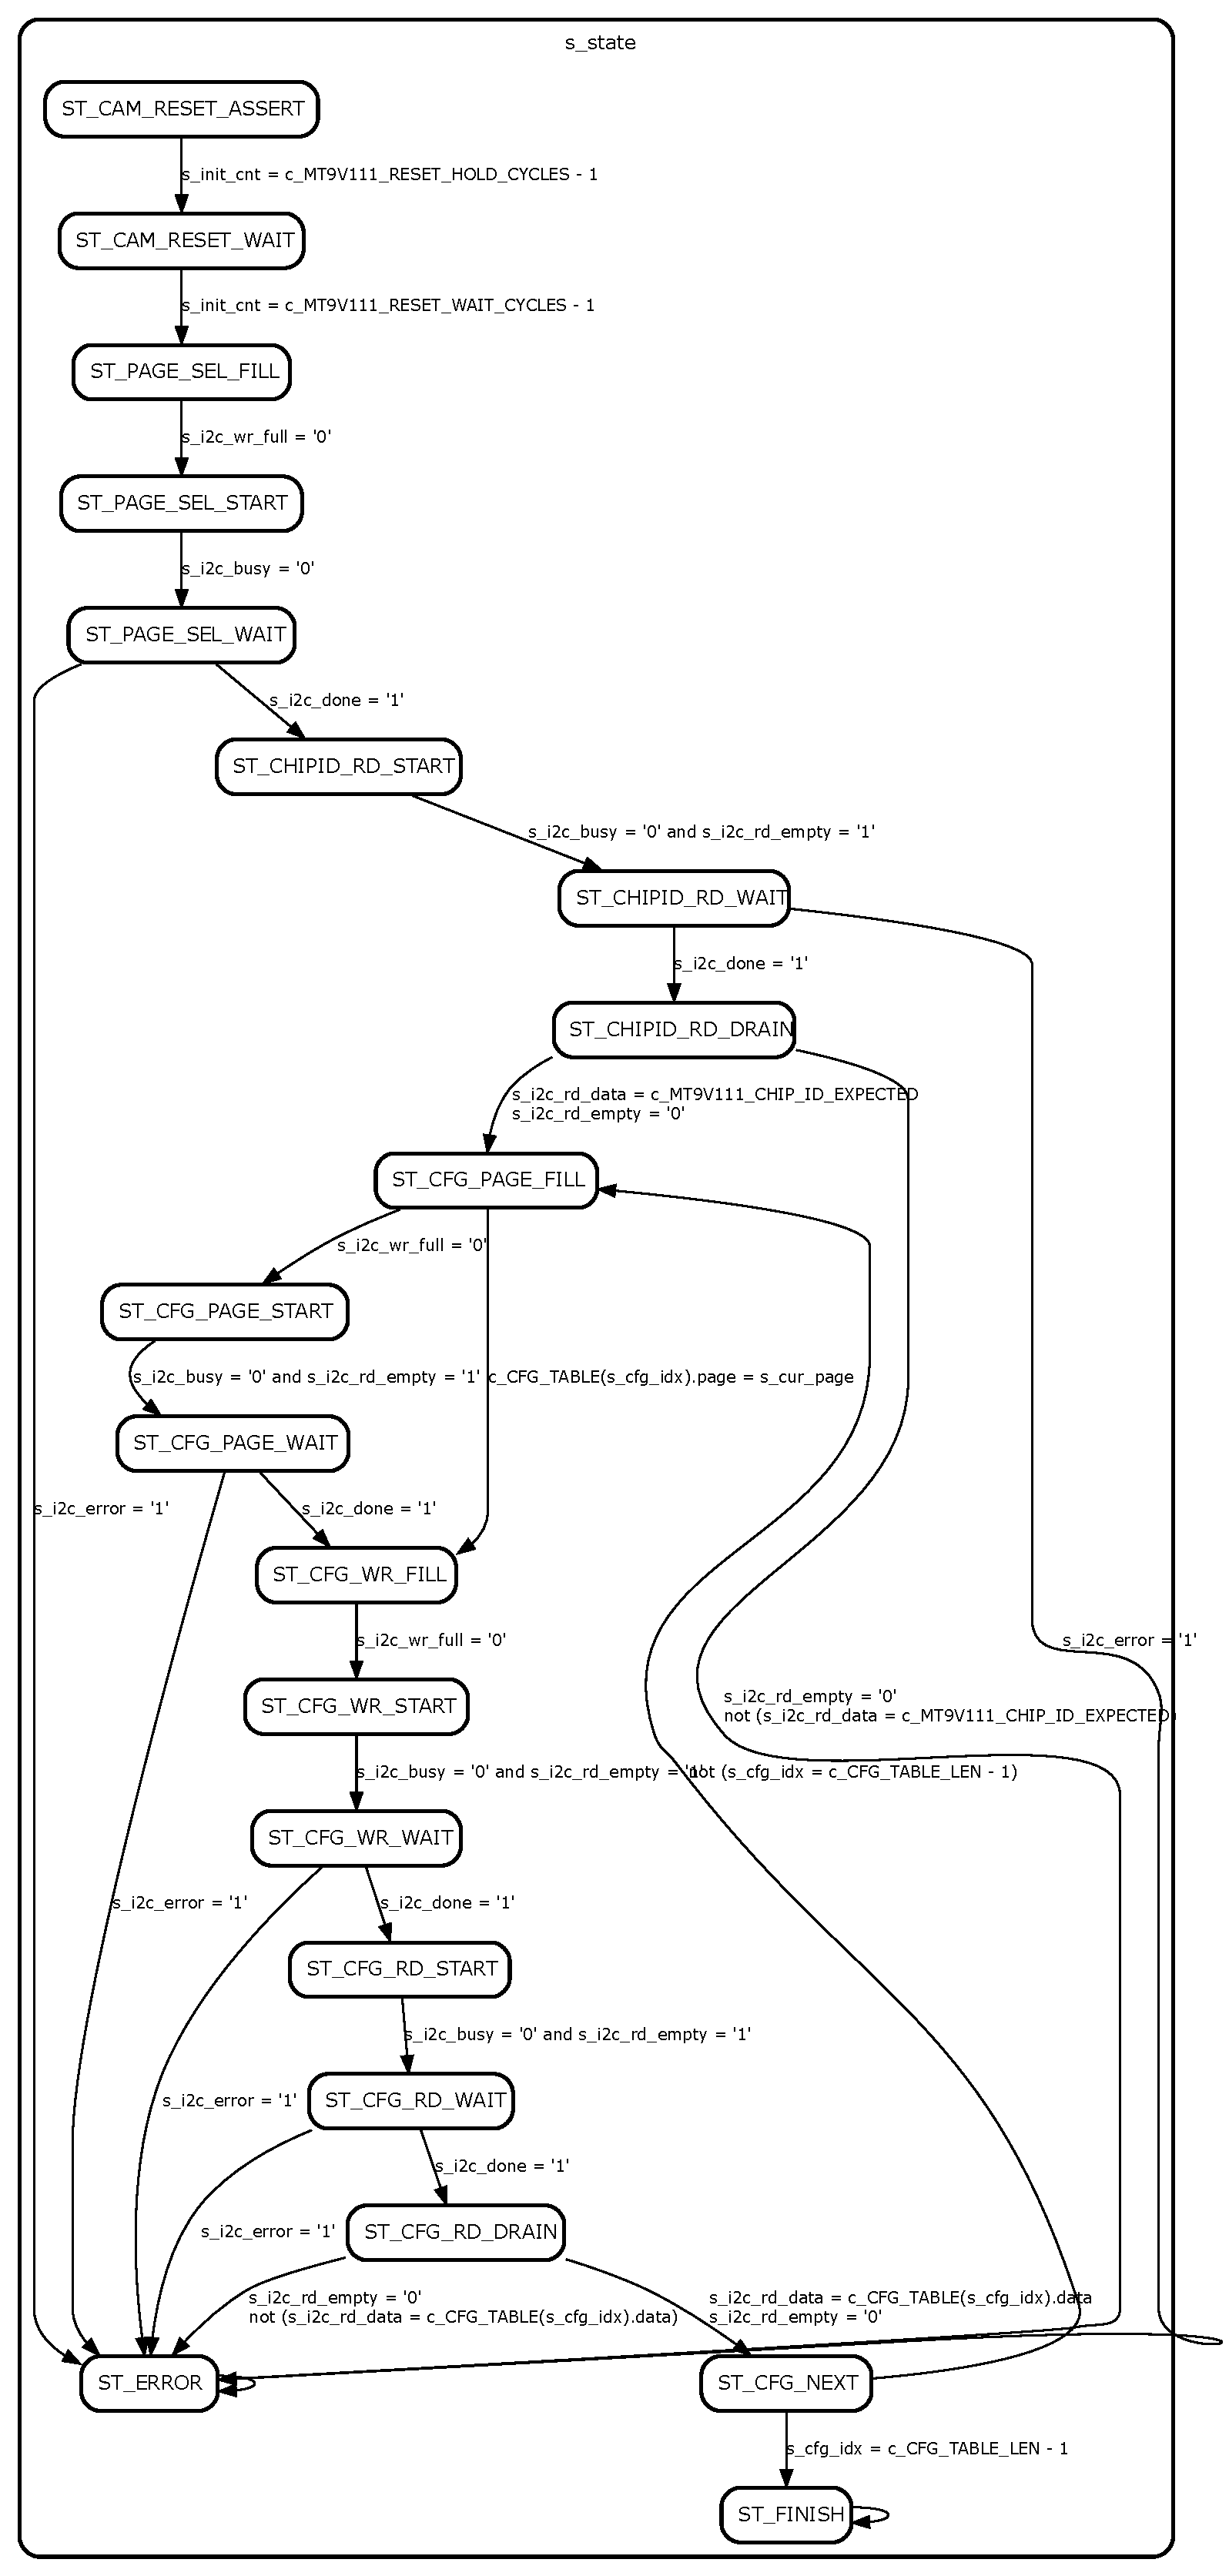
\includegraphics[width=0.7\textwidth]{gfx/anexo_fsm/fsm_top.pdf}
    \caption{FSM de configuración del sensor en \texttt{TOP.vhd}.}
    \label{fig:fsm_top}
\end{figure}

% -----------------------------------------------------------------
\section{FSM del \texttt{i2c\_controller}}
\label{sec:anexo_fsm_i2c}

Diagrama de estados completo del maestro \ac{I2C} \texttt{i2c\_controller.vhd} (37~estados, Tabla~\ref{tab:i2c_fsm}, Sección~\ref{sec:i2c_controller}).

\begin{figure}[htbp]
    \centering
    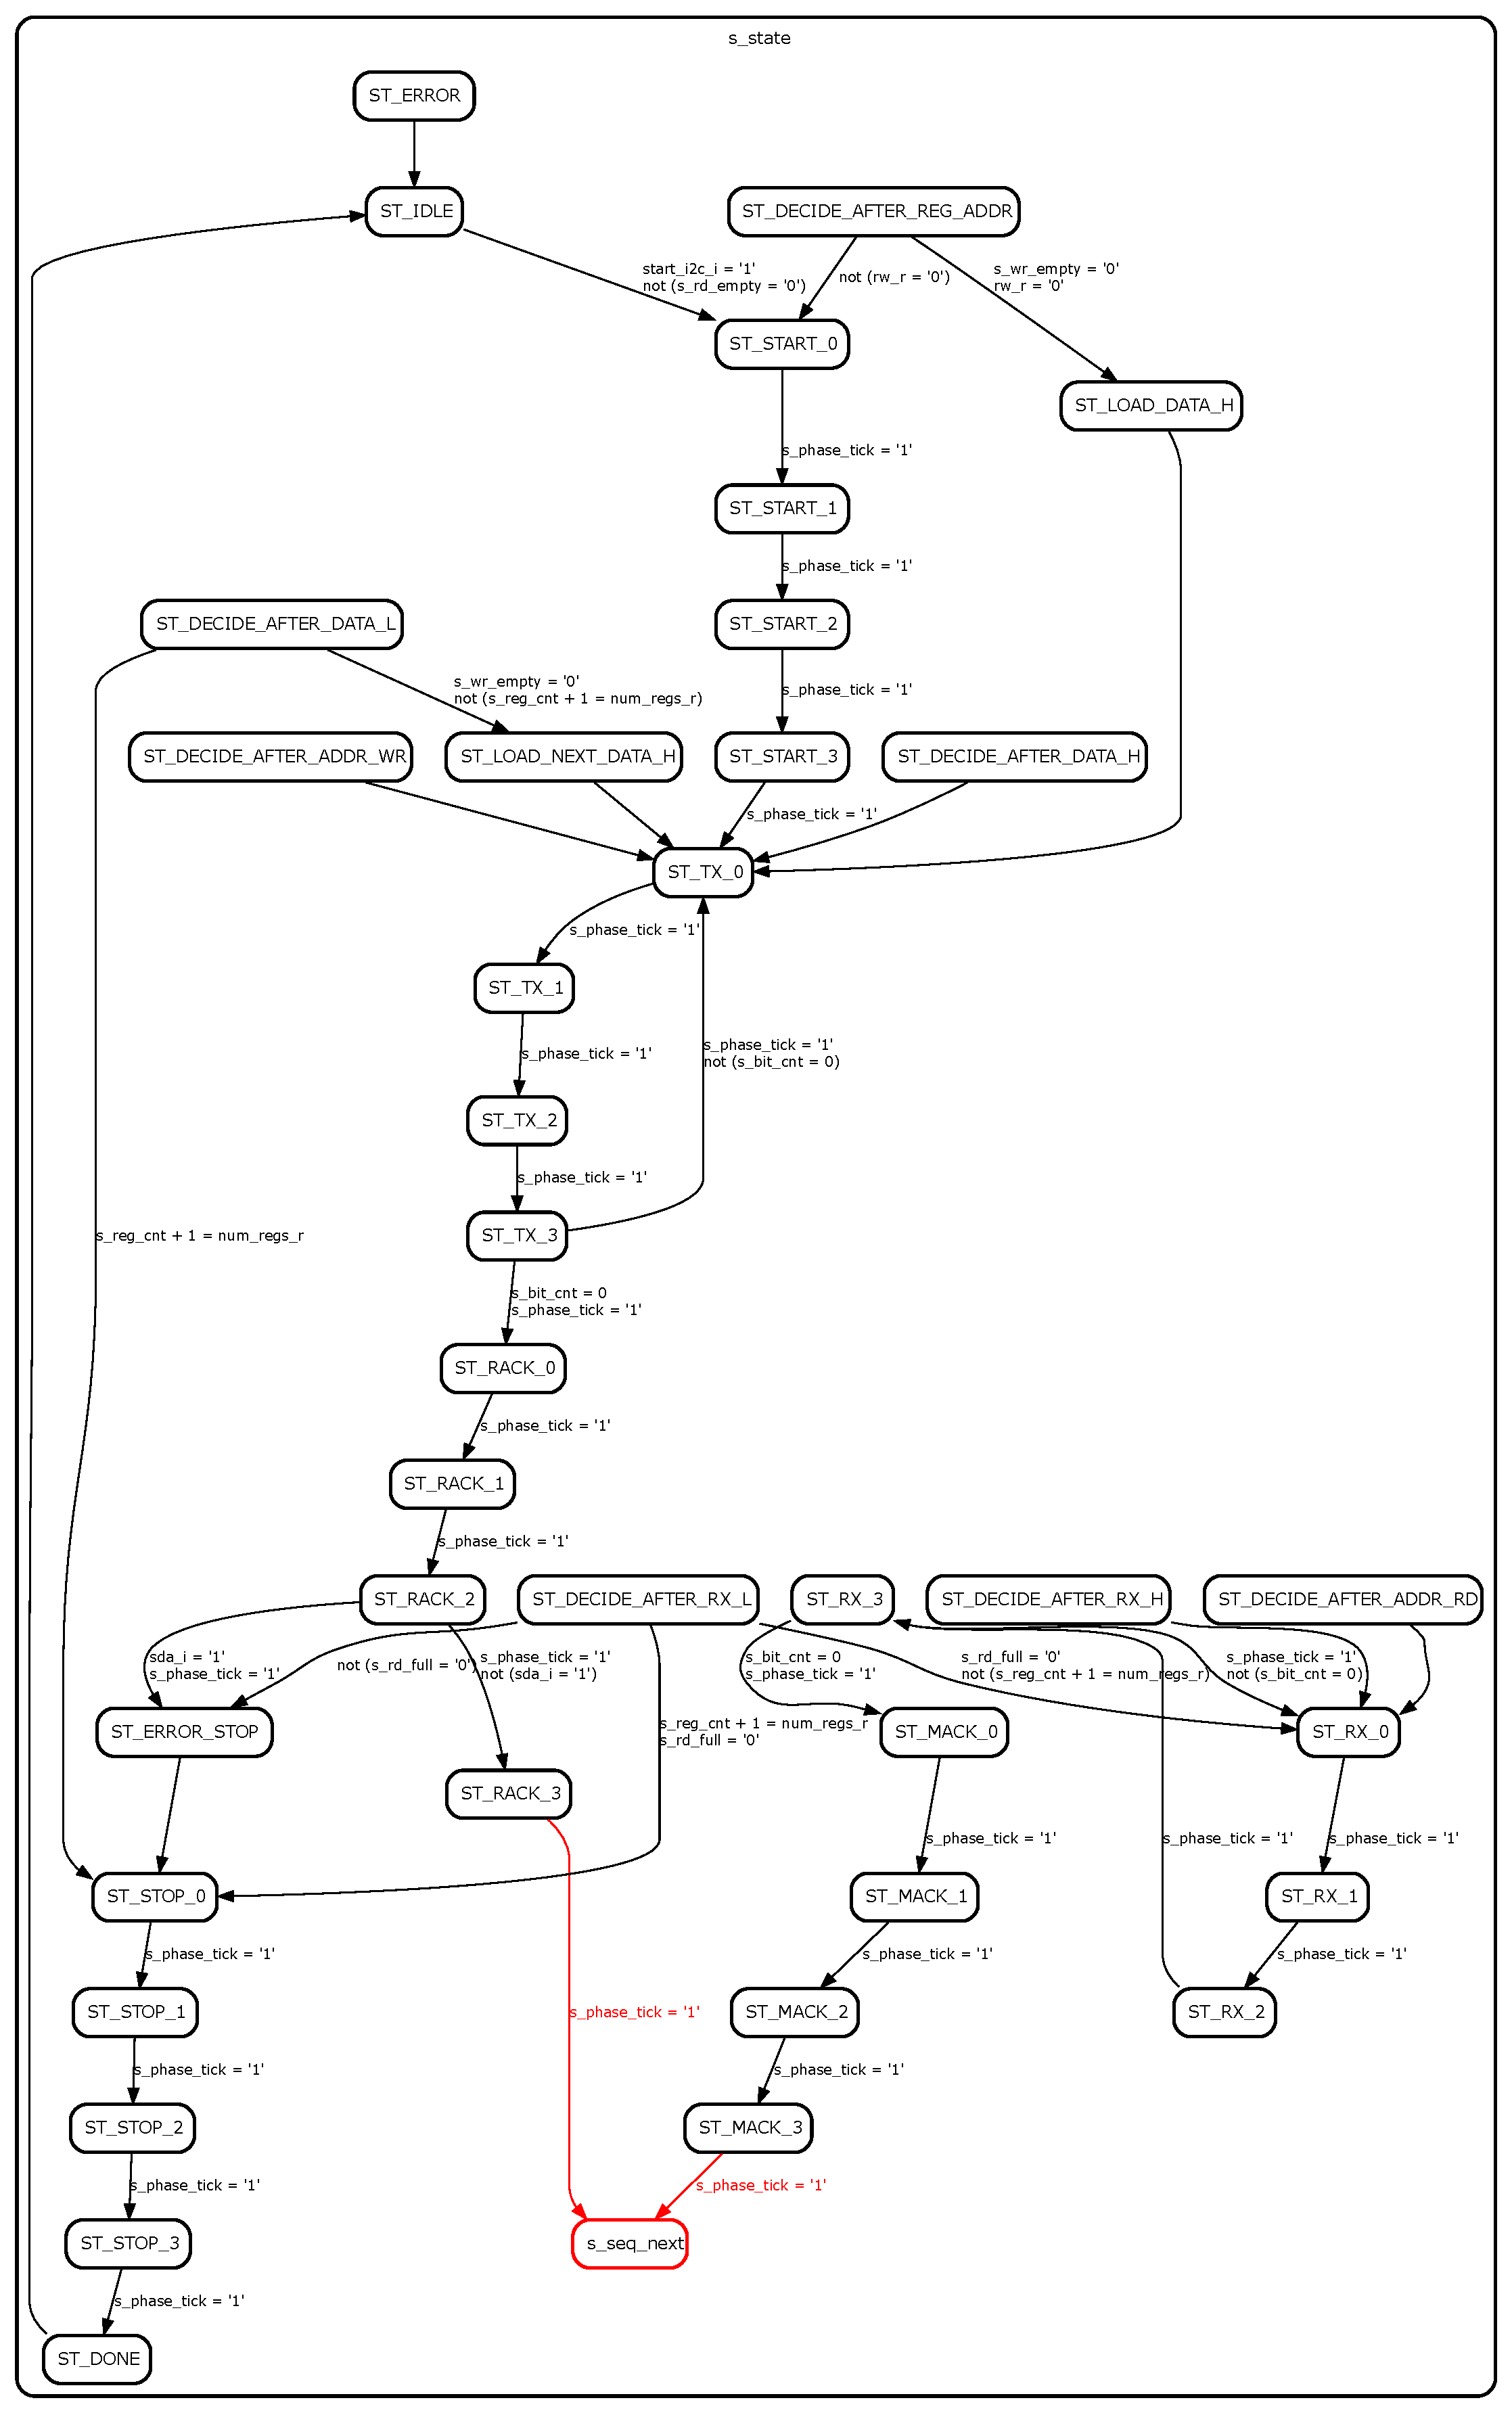
\includegraphics[width=0.7\textwidth]{gfx/anexo_fsm/fsm_i2c.pdf}
    \caption{FSM de \texttt{i2c\_controller.vhd}.}
    \label{fig:fsm_i2c}
\end{figure}

% -----------------------------------------------------------------
\section{FSM de recepción del \texttt{ftdi\_controller}}
\label{sec:anexo_fsm_ftdi}

Diagrama de estados del proceso \texttt{p\_rx} de \texttt{ftdi\_controller.vhd} (Sección~\ref{sec:ftdi_controller}), que gestiona la recepción de comandos PC$\rightarrow$FPGA en modo ráfaga continua.

\begin{figure}[htbp]
    \centering
    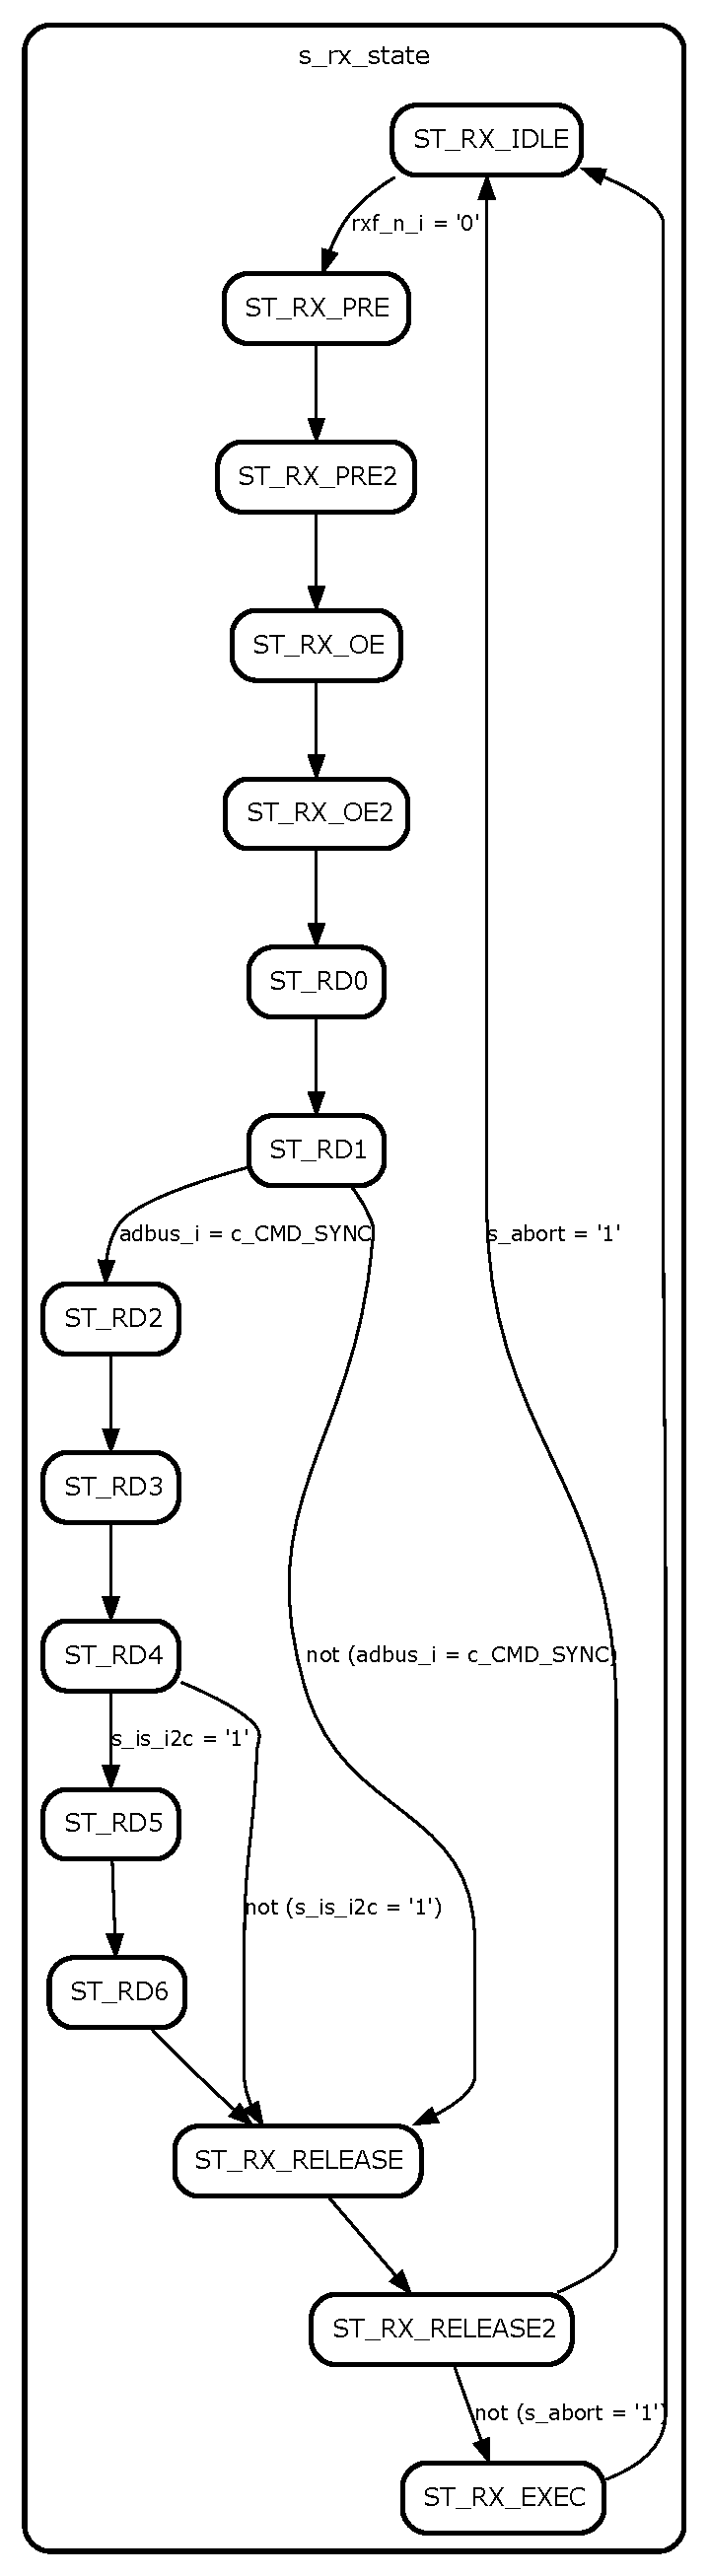
\includegraphics[width=0.35\textwidth]{gfx/anexo_fsm/fsm_ftdi.pdf}
    \caption{FSM de recepción (\texttt{p\_rx}) de \texttt{ftdi\_controller.vhd}.}
    \label{fig:fsm_ftdi_rx}
\end{figure}
 % Appendix B - empty
	%\include{Chapters/Chapter0C} %template
	%\include{Chapters/Chapter0D} %template
	\cleardoublepage
	\appendix
	\ctparttext{En esta parte se incluyen los manuales de usuario y documentación adicional.}
	\part{Apendices}

	\chapter{Manual de Usuario}
\label{ch:manual_usuario}

En este apéndice se detalla el manual de usuario correspondiente al sistema desarrollado, guiando paso a paso en el proceso de uso de la plataforma. Se asume que la \ac{FPGA} ya tiene el diseño programado en su memoria de configuración; este manual cubre por tanto la puesta en marcha del hardware y el uso del software de PC.

% -----------------------------------------------------------------
\section{Requisitos del sistema}
\label{sec:requisitos}

Antes de iniciar la instalación, hay que cumplir con los siguientes requisitos previos en su equipo:

\begin{itemize}
    \item \textbf{Sistema operativo:} Windows~11, con un mínimo de 8~GB de RAM.
    \item \textbf{Basys~3:} Basys~3 con el \textit{bitstream} de VICON ya programado en su memoria de configuración, conectada al sensor MT9V111 y al chip FT232H (módulo UM232H-B) utilizando los conectores \textit{Pmod} indicados en la Figura~\ref{fig:arq_fisica}.
    \item \textbf{Driver D2XX:} controlador D2XX de FTDI instalado en el PC (disponible en \url{https://ftdichip.com/drivers/d2xx-drivers/}), necesario para que la aplicación de PC acceda al FT232H.
    \item \textbf{Cable USB:} un cable USB~2.0 que conecte el módulo UM232H-B directamente a un puerto del PC. Se recomienda evitar conectarlo a través de un \textit{hub} USB, ya que puede introducir latencias adicionales en la recepción del vídeo.
\end{itemize}

\textit{Antes de encender o alimentar la placa}, comprobar la posición del \textit{jumper} de modo de arranque (\texttt{JP1}). Para que la Basys~3 cargue el diseño desde su memoria de configuración no volátil, dicho \textit{jumper} debe situarse en la posición \texttt{QSPI}; en la posición \texttt{USB} la placa esperaría en su lugar una programación por JTAG desde Vivado.

% -----------------------------------------------------------------
\section{Instalación y configuración}
\label{sec:instalacion}

Se deben seguir los pasos descritos a continuación para preparar el software de visualización:

\subsection{Descarga del código fuente}
Clonar el repositorio oficial del proyecto desde \url{https://github.com/carlosmgj/VICON}

\subsection{Configuración del módulo FT232H}
El módulo UM232H-B debe tener su \ac{EEPROM} configurada en modo \textbf{FT245 FIFO} para poder operar en modo \textit{Synchronous FIFO}. Esta configuración solo es necesaria una vez por dispositivo:

\begin{enumerate}
    \item Instalar la utilidad \textbf{FT\_Prog} de FTDI (requiere el driver D2XX ya instalado).
    \item Conectar el UM232H-B al PC y, en FT\_Prog, pulsar \textit{Scan and Parse} para detectar el dispositivo.
    \item Navegar hasta \texttt{FT EEPROM~$\rightarrow$~Hardware Specific~$\rightarrow$~Port~A~$\rightarrow$~Hardware} y cambiar el modo de \texttt{UART} a \texttt{245~FIFO}.
    \item Programar la \ac{EEPROM} (icono del rayo) y, al finalizar, desconectar y vuelva a conectar el módulo para que el sistema operativo lo reconozca con la nueva configuración.
\end{enumerate}

\subsection{Compilación de la aplicación de PC}
La aplicación \texttt{vicon\_view} se distribuye como un ejecutable y por tanto no hace falta tener las dependencias instaladas. Únicamente serían necesarias para la compilación de la aplicación.
La ruta del ejecutable es: \url{VICON/07-Versions/3.0/GUI/vicon_gui.exe}
% -----------------------------------------------------------------
\section{Guía de uso de la aplicación}
\label{sec:guia_uso}

\subsection{Inicio de la aplicación}
Con la Basys~3 encendida, el sensor conectado y el módulo FT232H enlazado al PC por USB, ejecutar \texttt{vicon\_view}. La aplicación abre el dispositivo FT232H a través del \textit{driver} D2XX y comienza a recibir el flujo de vídeo sintético de forma automática; no es necesario ningún paso adicional de emparejamiento o configuración del enlace.

\subsection{Descripción de la interfaz}
Una vez iniciada la interfaz de usuario, se presentan dos zonas principales:

\begin{enumerate}
    \item \textbf{Ventana de vídeo:} muestra en tiempo real el fotograma recibido desde la \ac{FPGA} en escala de grises, junto con la tasa de fotogramas por segundo (\ac{FPS}) actual.
    \item \textbf{Panel de control:} Se encuentran los controles para enviar comandos a la \ac{FPGA}, descritos en la Tabla~\ref{tab:comandos_gui}.
\end{enumerate}

Por defecto, la interfaz muestra el video sintético generado para validar la comunicación entre el sensor y el Host a través de la FPGA como se ve en la Figura~\ref{fig:GUI1}:

\begin{figure}[htbp]
    \centering
    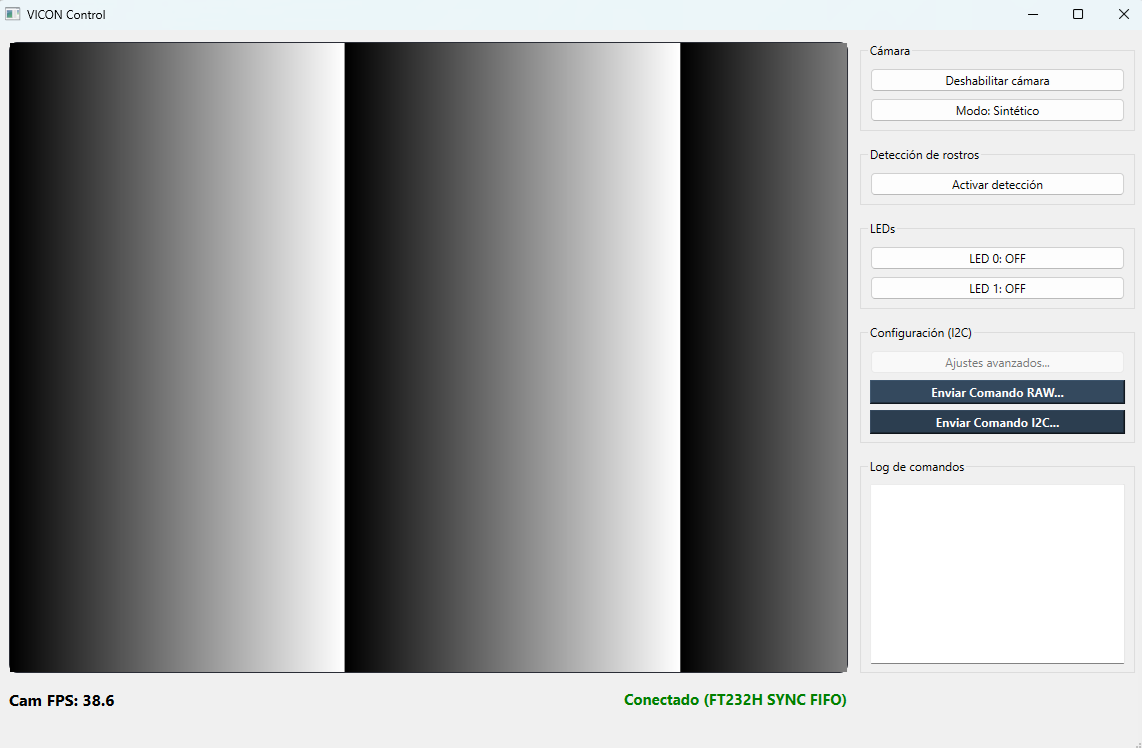
\includegraphics[width=\textwidth]{gfx/vicon_view_gui1.png}
    \caption{Estado Inicial de la Interfaz Gráfica de Usuario.}
    \label{fig:GUI1}
\end{figure}

Para configurar los FPS de la imágen a mínimo 30fps, se deberá configurar el registro I2C correspondiente mandando la trama 1 0x37 0x0080 (Ver Figura~\ref{fig:GUI2}). Este paso se puede realizar antes o después de cambiar el modo de la imágen. 

\begin{figure}[htbp]
    \centering
    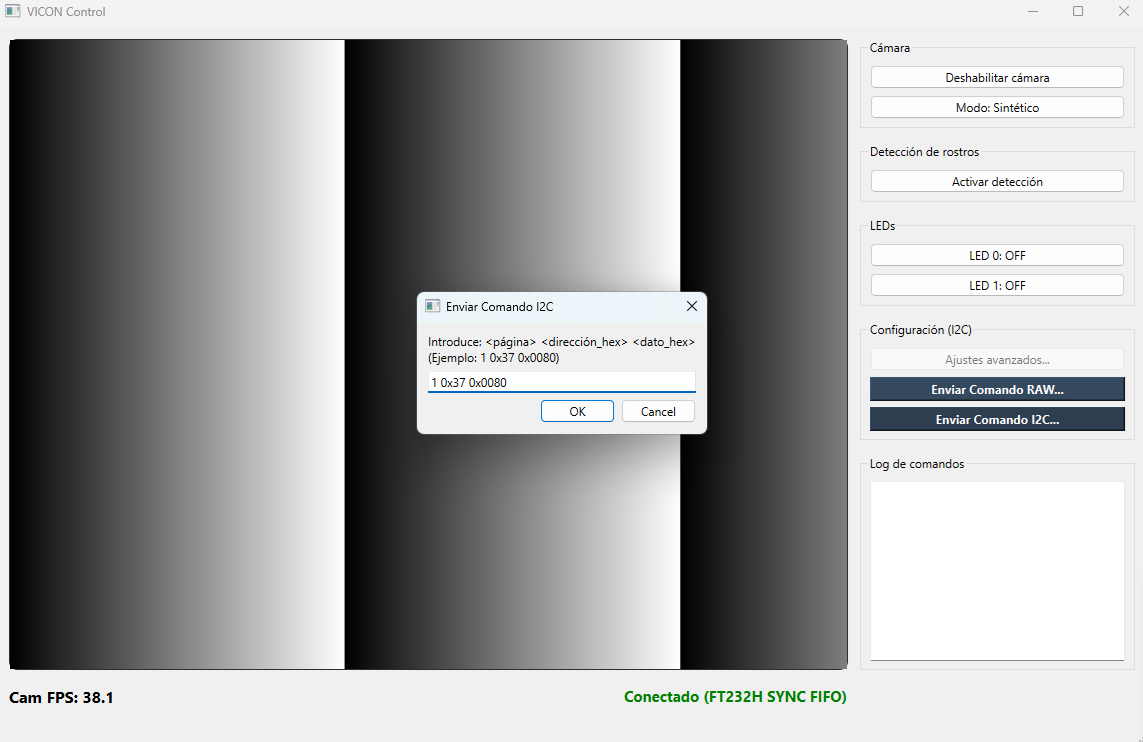
\includegraphics[width=\textwidth]{gfx/vicon_view_gui2.png}
    \caption{GUI: envío de comando I2C para configurar >30fps.}
    \label{fig:GUI2}
\end{figure}

Si a continuación habilitamos la imagen del sensor real y la detección de rostros, el software remarcara la/s cara/s que detecte en la imagen. En la Figura~\ref{fig:GUI3} se puede ver el resultado de presentar al sensor una foto en una tablet con múltiples caras. 

\begin{figure}[htbp]
    \centering
    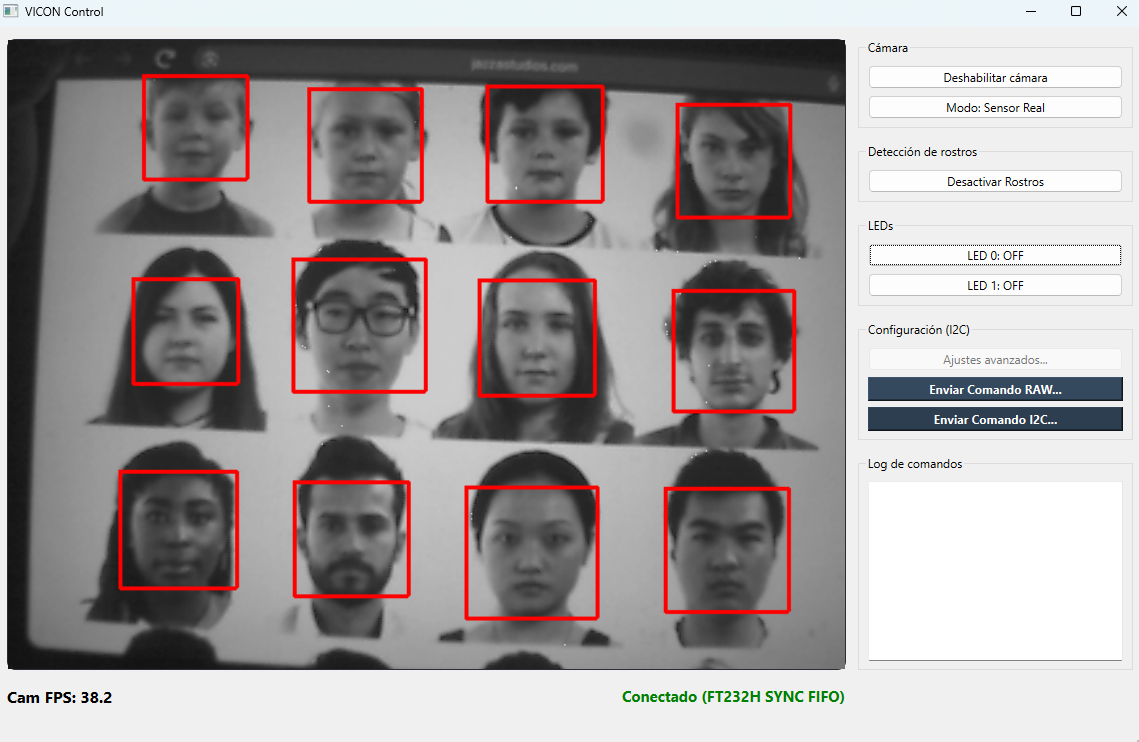
\includegraphics[width=\textwidth]{gfx/vicon_view_gui3.png}
    \caption{GUI: envío de comando I2C para configurar >30fps.}
    \label{fig:GUI3}
\end{figure}

\begin{table}[H]
\centering
\caption{Comandos disponibles desde la interfaz de \texttt{vicon\_view}.}
\label{tab:comandos_gui}
\begin{tabular}{>{\raggedright\arraybackslash}p{3cm}>{\raggedright\arraybackslash}p{9.5cm}}
\rowcolor[HTML]{156082}
{\color{white}\textbf{Comando}} & {\color{white}\textbf{Efecto}} \\
\rowcolor[HTML]{C0E6F5}
LED & Conmuta el estado de un LED de la Basys~3, útil como comprobación rápida de que el canal de comandos PC$\rightarrow$FPGA funciona. \\
Activar/desactivar captura & Detiene o reanuda la transmisión de vídeo desde la \ac{FPGA} sin necesidad de desconectar el enlace USB. \\
\rowcolor[HTML]{C0E6F5}
Imagen sintética & Conmuta entre el sensor MT9V111 y el generador interno de imagen sintética, útil para validar el resto de la cadena sin depender de la cámara física. \\
Escritura de registro I2C & Permite escribir un valor en un registro concreto del sensor (página, dirección y dato), para ajustar su configuración en caliente. \\
\end{tabular}
\end{table}

% -----------------------------------------------------------------
\section{Resolución de problemas (\textit{troubleshooting})}
\label{sec:problemas}

En la Tabla~\ref{tab:errores_frecuentes} se resumen los errores más habituales y las acciones recomendadas para su resolución.

\begin{table}[htbp]
\centering
\caption{Problemas frecuentes y soluciones.}
\label{tab:errores_frecuentes}
\begin{tabular}{|p{3.8cm}|p{4.6cm}|p{4.6cm}|}
\hline
\rowcolor[HTML]{156082}
{\color{white}\textbf{Error}} & {\color{white}\textbf{Causa probable}} & {\color{white}\textbf{Solución recomendada}} \\ \hline
No se ven los LEDs encendidos al arrancar la placa. & \textit{Jumper} de modo mal colocado. & Situar el \textit{jumper} \texttt{JP1} en modo \texttt{QSPI} antes de alimentar la placa. \\ \hline
La aplicación no detecta el FT232H. & Windows ha instalado automáticamente el \textit{driver} VCP (puerto serie virtual) en lugar del D2XX. & Reinstalar el \textit{driver} D2XX desde el Administrador de dispositivos, seleccionando manualmente la carpeta de instalación de FTDI. \\ \hline
FT\_Prog no reconoce el dispositivo al configurar la \ac{EEPROM}. & Conflicto entre el \textit{driver} D2XX y otro \textit{driver} (p.~ej. \texttt{libusb}) instalado previamente sobre el mismo dispositivo. & Reinstalar el \textit{driver} D2XX y volver a conectar el cable antes de reintentar con FT\_Prog. \\ \hline
El vídeo se congela o aparecen fotogramas corruptos de forma intermitente. & Sobreescritura de la \ac{FIFO} interna por una latencia de lectura excesiva en el PC (agravada si el FT232H está conectado a través de un \textit{hub} USB). & Conectar el módulo directamente a un puerto USB del equipo, sin \textit{hubs} intermedios. \\ \hline
\end{tabular}
\end{table}
	\cleardoublepage
	\chapter{Diagramas de estados (FSM)}
\label{ch:anexo_fsm}

Este anexo recoge los diagramas de estados completos de las máquinas de estados finitas (\ac{FSM}) más voluminosas del diseño, referenciadas desde sus respectivos módulos en el Capítulo~\ref{chap:desarrollo}. Se han trasladado aquí, en lugar de incluirse en el cuerpo del documento, debido a su tamaño.

% -----------------------------------------------------------------
\section{FSM de configuración del TOP}
\label{sec:anexo_fsm_top}

Diagrama de estados de la FSM principal \texttt{p\_fsm} (\texttt{TOP.vhd}), descrita textualmente en la Sección~\ref{sec:top}.

\begin{figure}[htbp]
    \centering
    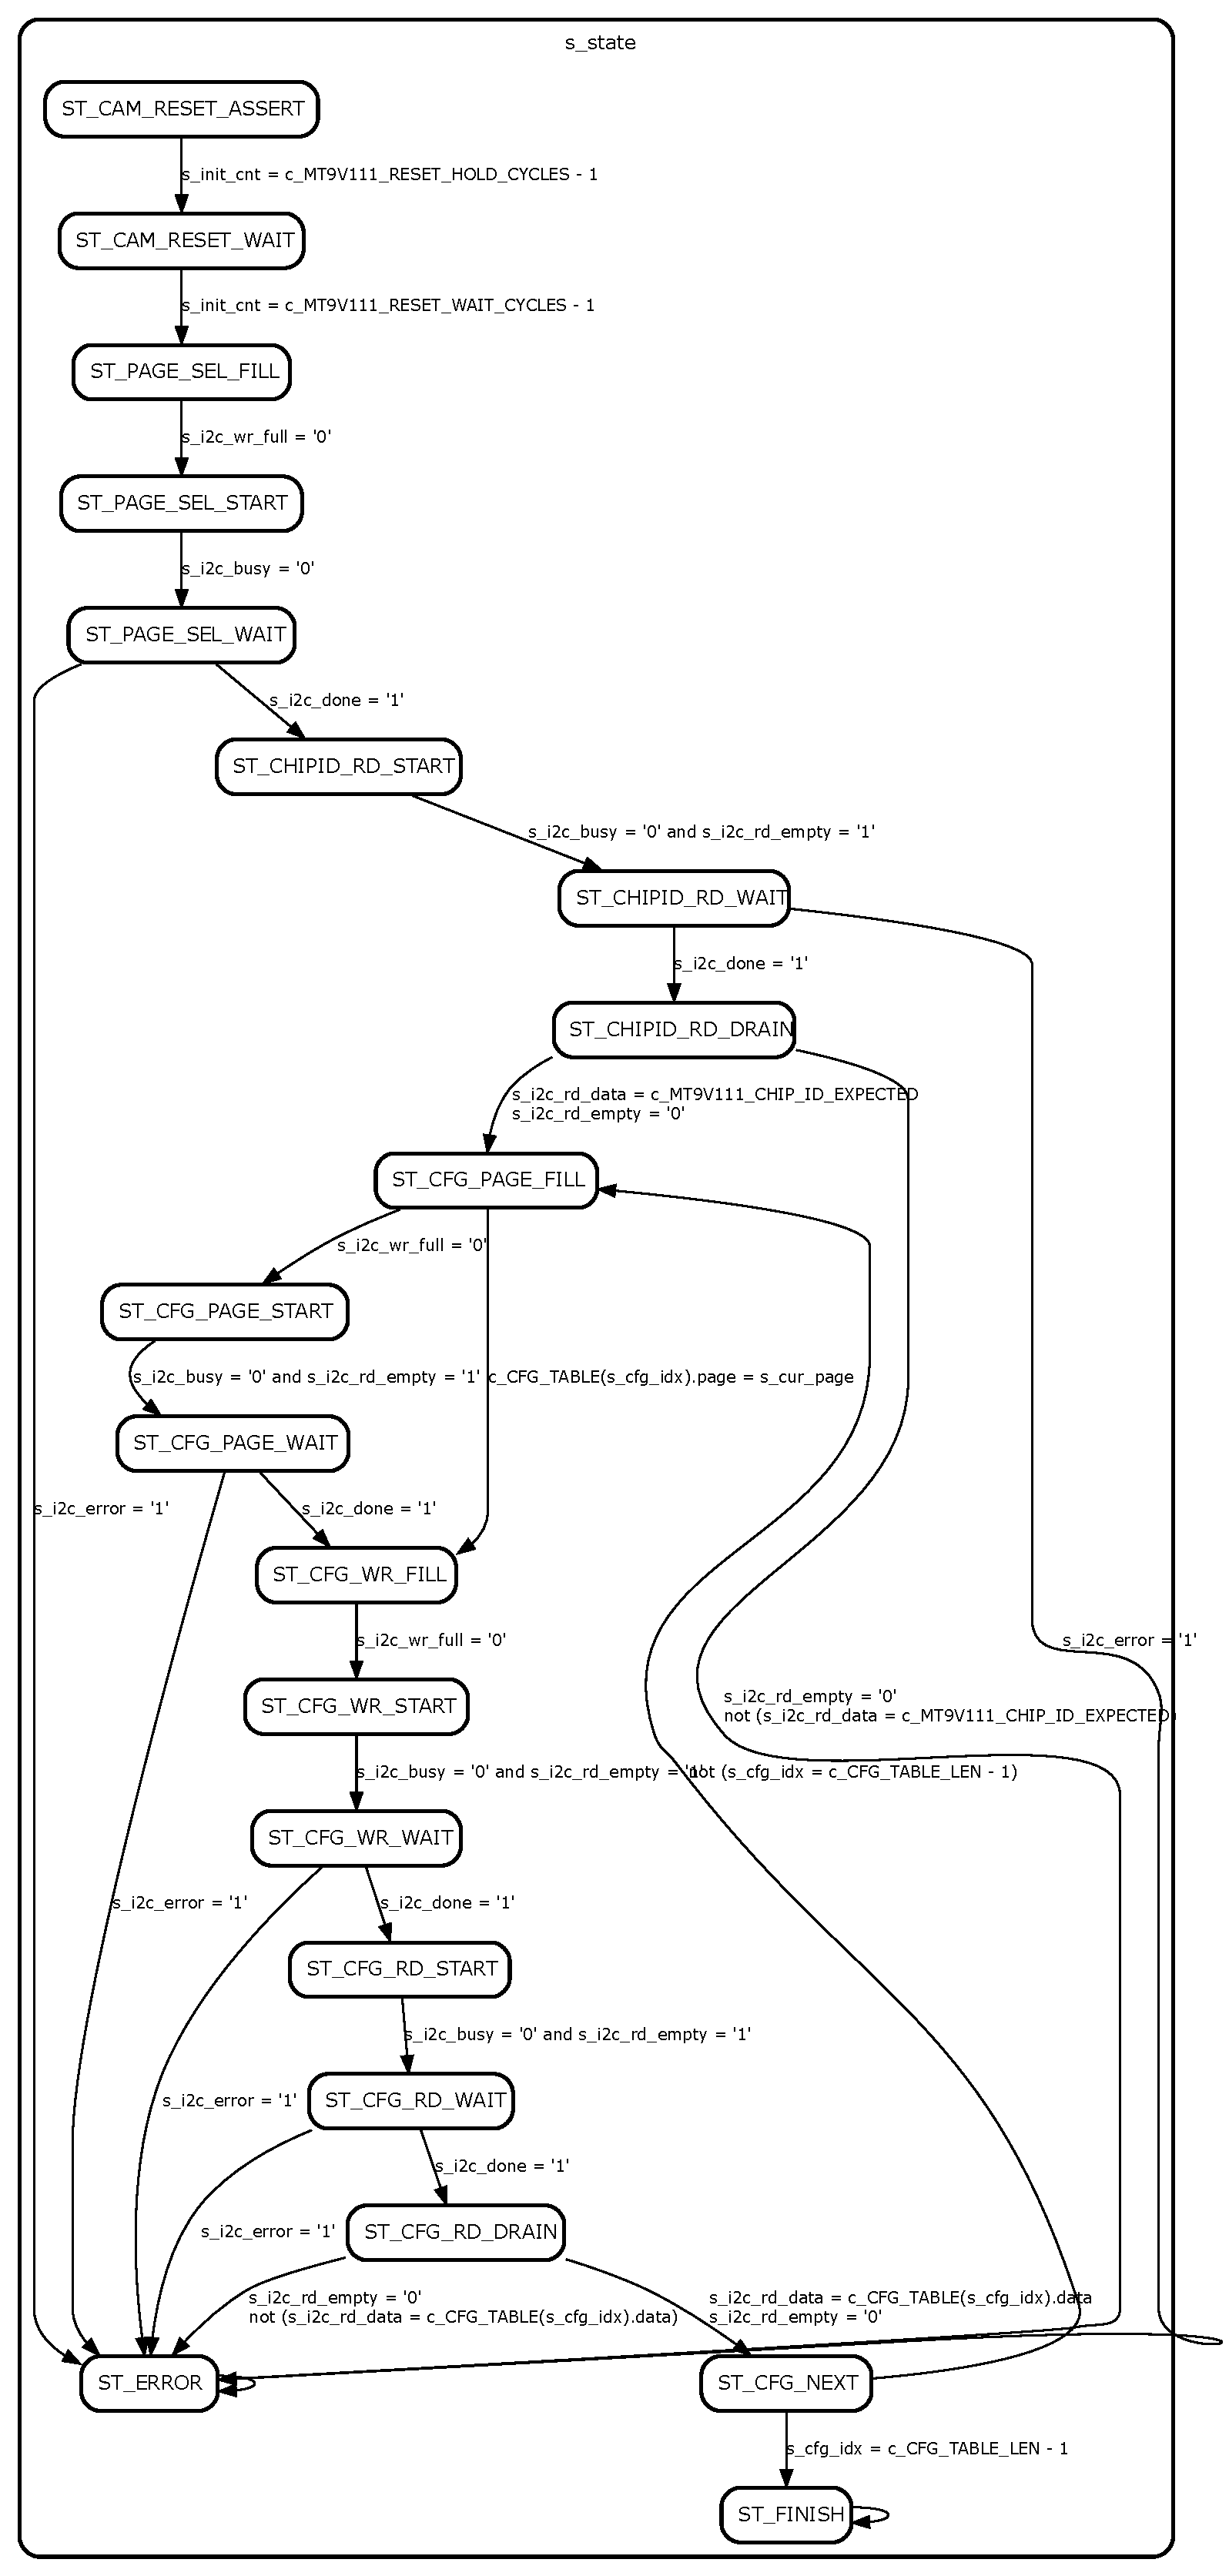
\includegraphics[width=0.7\textwidth]{gfx/anexo_fsm/fsm_top.pdf}
    \caption{FSM de configuración del sensor en \texttt{TOP.vhd}.}
    \label{fig:fsm_top}
\end{figure}

% -----------------------------------------------------------------
\section{FSM del \texttt{i2c\_controller}}
\label{sec:anexo_fsm_i2c}

Diagrama de estados completo del maestro \ac{I2C} \texttt{i2c\_controller.vhd} (37~estados, Tabla~\ref{tab:i2c_fsm}, Sección~\ref{sec:i2c_controller}).

\begin{figure}[htbp]
    \centering
    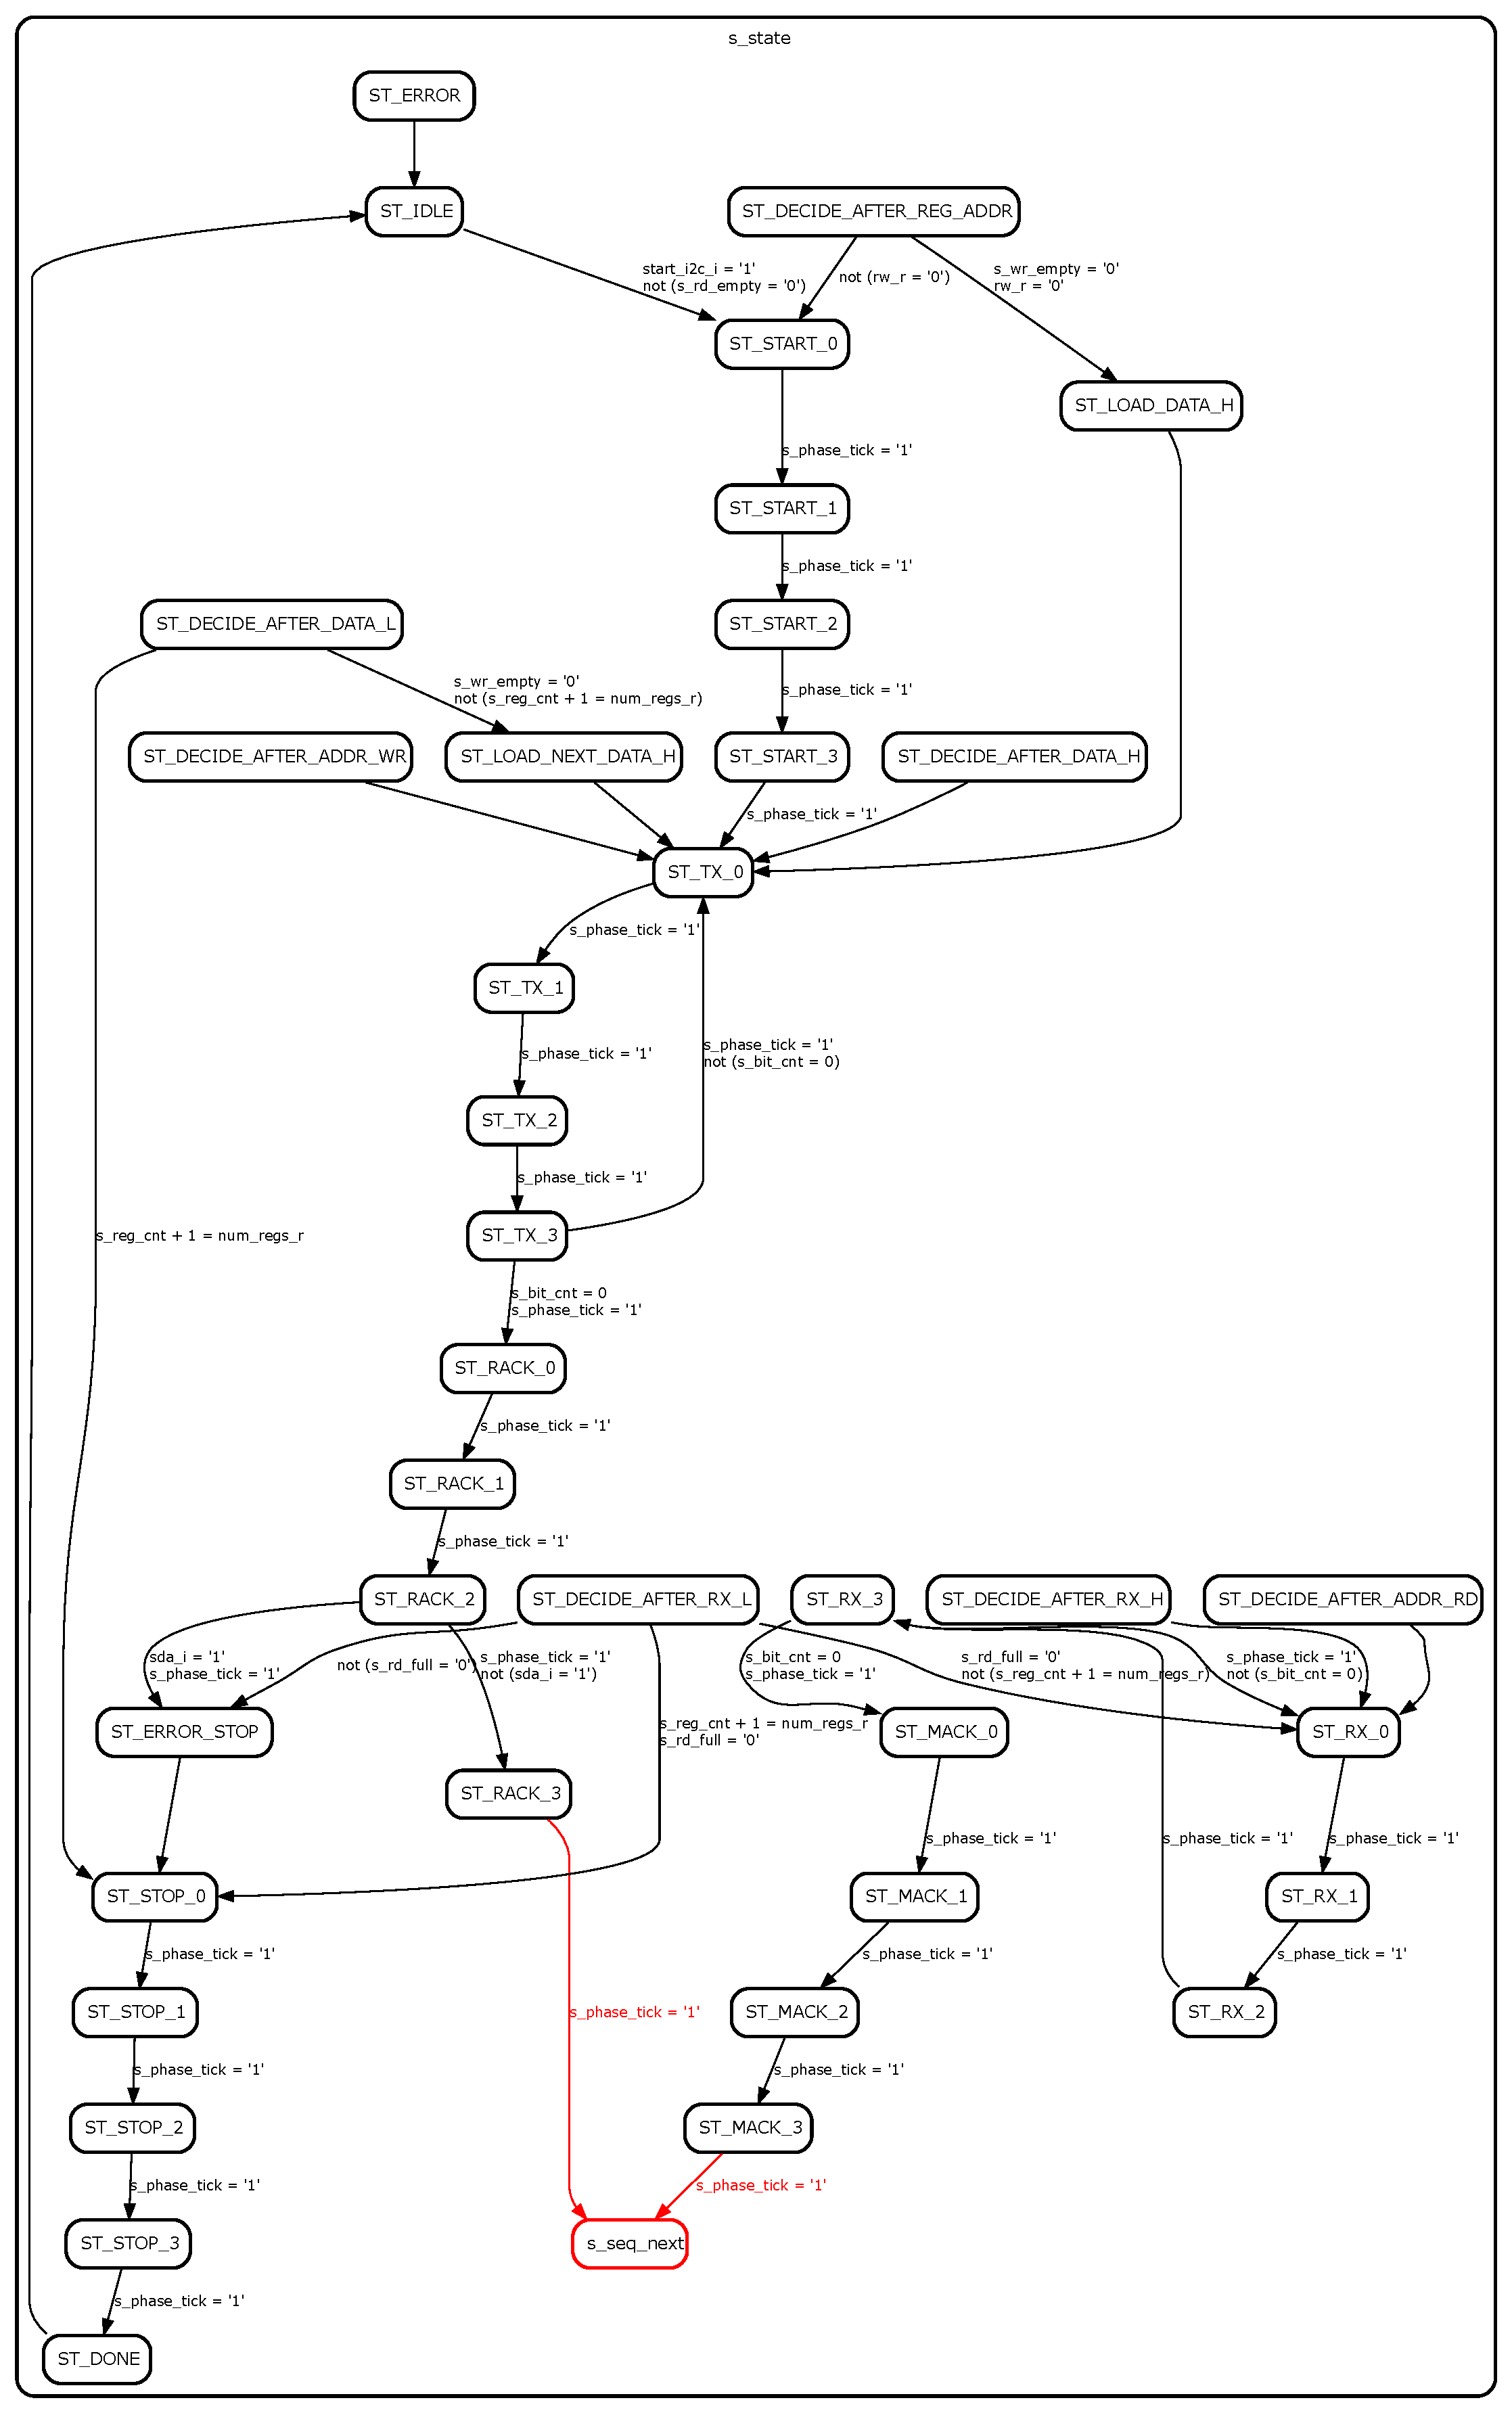
\includegraphics[width=0.7\textwidth]{gfx/anexo_fsm/fsm_i2c.pdf}
    \caption{FSM de \texttt{i2c\_controller.vhd}.}
    \label{fig:fsm_i2c}
\end{figure}

% -----------------------------------------------------------------
\section{FSM de recepción del \texttt{ftdi\_controller}}
\label{sec:anexo_fsm_ftdi}

Diagrama de estados del proceso \texttt{p\_rx} de \texttt{ftdi\_controller.vhd} (Sección~\ref{sec:ftdi_controller}), que gestiona la recepción de comandos PC$\rightarrow$FPGA en modo ráfaga continua.

\begin{figure}[htbp]
    \centering
    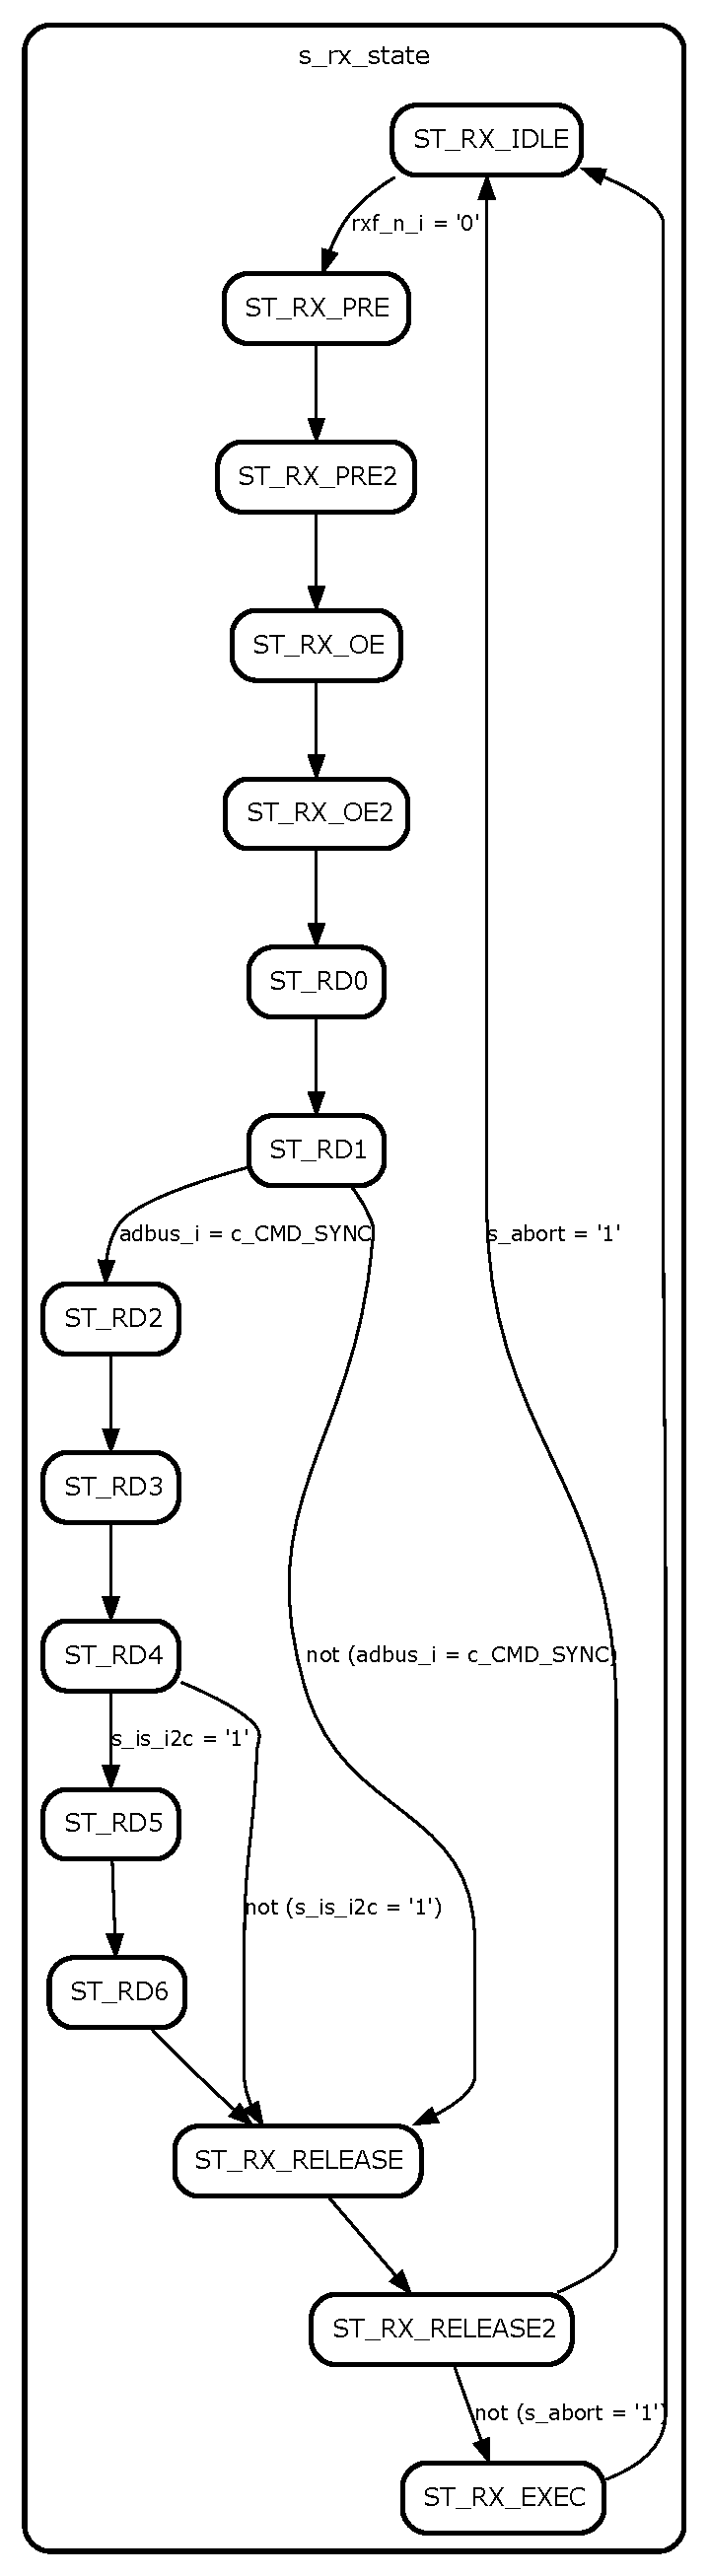
\includegraphics[width=0.35\textwidth]{gfx/anexo_fsm/fsm_ftdi.pdf}
    \caption{FSM de recepción (\texttt{p\_rx}) de \texttt{ftdi\_controller.vhd}.}
    \label{fig:fsm_ftdi_rx}
\end{figure}

	%----------------------------------------------------------------------------------------
	%	POST-CONTENT THESIS PAGES
	%----------------------------------------------------------------------------------------
	
    
	%1\cleardoublepage\include{FrontBackMatter/Colophon} % Colophon
	
	%1\cleardoublepage\include{FrontBackMatter/Declaration} % Declaration
	
	%1\cleartoleftpage\include{FrontBackMatter/Backpage} % Back cover
	%----------------------------------------------------------------------------------------
	

\end{document}